% !TeX program = pdflatex
% !TeX encoding = UTF-8
% 香港大学 Capstone 期末报告框架。正文使用英文，中文仅用于源码注释。
% 先修改下方封面资料，再搜索 TODO，逐项替换写作提示。
% 参考排版：Capstone_Final_Report_Ref.pdf；不是学校官方模板。
\documentclass[12pt,a4paper,oneside]{report}

% ==================== 页面与字体 ====================
\usepackage[a4paper,margin=1in]{geometry}
% 保留默认 Computer Modern 字体，与参考 PDF 的字体一致。
\usepackage[utf8]{inputenc}
\usepackage{amsmath,amssymb}
\usepackage{graphicx}
\usepackage{booktabs,tabularx,longtable,array}
\usepackage{xcolor}
\usepackage{makecell,multirow}
\usepackage{caption}
\usepackage{placeins}
\usepackage{etoolbox}
\usepackage{enumitem}
\usepackage{setspace}
\usepackage[authoryear,square]{natbib}
\usepackage[hidelinks]{hyperref}
\usepackage{xurl}
\graphicspath{{figures/}}
\setstretch{1.25} % 12pt 正文的行距约 18pt，按参考 PDF 估计。
\setlength{\parindent}{1.5em}
\setlength{\parskip}{0pt}
\setlength{\emergencystretch}{2em}
\pagestyle{plain} % 无页眉，页码位于页脚中间。
\setcounter{secnumdepth}{2}
\setcounter{tocdepth}{2}
\setlist{topsep=0.5\baselineskip,itemsep=0.25\baselineskip}
\newcolumntype{Y}{>{\raggedright\arraybackslash}X}

% ==================== TODO：封面资料 ====================
\newcommand{\UniversityName}{The University of Hong Kong}
\newcommand{\FacultyName}{Faculty of Science}
\newcommand{\ProgrammeName}{Master of Science in Artificial Intelligence Programme}
\newcommand{\CourseName}{ARIN7600 Artificial Intelligence Project}
\newcommand{\CourseSession}{[Year/Term]}
\newcommand{\ProjectTitle}{[Your Project Title]}
% 多人可用逗号分隔，太长时可在合适位置加入 \\ 换行。
\newcommand{\StudentNames}{[Student Name] ([Student ID])}
\newcommand{\PrimarySupervisor}{[Primary Supervisor Name]}
\newcommand{\SecondarySupervisor}{[Secondary Supervisor Name]}
\newcommand{\SubmissionDate}{[YYYY/MM/DD]}

% 默认显示参考报告末尾的可编辑分工表；不需要时改成 false。
\newif\ifincludeworkdistribution
\includeworkdistributiontrue
% 参考文献由 chapters/references.tex 生成。

\hypersetup{
  pdftitle={\ProjectTitle},
  pdfauthor={\StudentNames},
  pdfsubject={ARIN7600 Final Report}
}

% ==================== 章标题与辅助命令 ====================
% 模仿参考：Chapter N 与章名分两行、居中、粗体。
\makeatletter
\renewcommand{\@makechapterhead}[1]{%
  \vspace*{50\p@}%
  {\parindent\z@\centering\normalfont
    \ifnum\c@secnumdepth>\m@ne
      \Huge\bfseries \@chapapp\space\thechapter\par\nobreak
      \vskip20\p@
    \fi
    \interlinepenalty\@M
    \Huge\bfseries #1\par\nobreak
    \vskip40\p@}}
\renewcommand{\@makeschapterhead}[1]{%
  \vspace*{50\p@}%
  {\parindent\z@\centering\normalfont
    \interlinepenalty\@M
    \Huge\bfseries #1\par\nobreak
    \vskip40\p@}}
% 目录保留左对齐标题，与参考报告一致。
\newcommand{\ReportContents}{%
  \begingroup
  \renewcommand{\@makeschapterhead}[1]{%
    \vspace*{50\p@}%
    {\parindent\z@\raggedright\normalfont
     \Huge\bfseries ##1\par\nobreak\vskip40\p@}}%
  \tableofcontents
  \endgroup}
\makeatother

% 不编号的章也自动进入目录，页码随编译更新。
\newcommand{\unnumberedchapter}[1]{%
  \chapter*{#1}%
  \phantomsection
  \addcontentsline{toc}{chapter}{#1}}
\renewcommand{\bibsection}{\unnumberedchapter{References}}
\setlength{\bibhang}{1em}

% 可见的写作占位提示。写作时将整个 \placeholder{...} 替换成正文。
\newcommand{\placeholder}[1]{{\color{gray}[#1]}}
\newcommand{\figureplaceholder}[2][45mm]{%
  \fbox{\parbox[c][#1][c]{0.90\linewidth}{%
    \centering\color{gray}#2}}}


% Single-column report adapters for the migrated manuscript tables and floats.
\captionsetup{font=small,labelfont=normalfont}
\newsavebox{\reporttablebox}
\newenvironment{fittable}{\begin{lrbox}{\reporttablebox}}{%
  \end{lrbox}%
  \ifdim\wd\reporttablebox>\linewidth
    \typeout{REPORT TABLE SCALED: natural=\the\wd\reporttablebox; target=\the\linewidth}%
    \resizebox{\linewidth}{!}{\usebox{\reporttablebox}}%
  \else\usebox{\reporttablebox}\fi}
\AtBeginEnvironment{table}{\singlespacing}
\setcounter{topnumber}{3}
\setcounter{bottomnumber}{2}
\setcounter{totalnumber}{5}
\renewcommand{\topfraction}{0.9}
\renewcommand{\bottomfraction}{0.85}
\renewcommand{\textfraction}{0.08}
\renewcommand{\floatpagefraction}{0.65}
\raggedbottom

\begin{document}

% ==================== 封面：不显示页码 ====================
\hypersetup{pageanchor=false}
\begin{titlepage}
\thispagestyle{empty}
\begin{center}
  \vspace*{2.45cm}
  {\LARGE \UniversityName\par}
  \vspace{0.35cm}
  {\Large \FacultyName\par}
  \vspace{0.35cm}
  {\Large \ProgrammeName\par}
  \vspace{1.3cm}
  {\large \CourseName\space\CourseSession\par}
  \vspace{0.9cm}
  {\Huge Final Report\par}
  \vspace{1.6cm}
  {\Large\bfseries Topic: \ProjectTitle\par}
  \vspace{1.6cm}
\end{center}
\noindent\textbf{Student:} \StudentNames\par
\noindent\textbf{Primary Supervisor:} \PrimarySupervisor\par
% 没有第二导师时可删除下一行。
\noindent\textbf{Secondary Supervisor:} \SecondarySupervisor\par
\noindent\textbf{Submission Date:} \SubmissionDate\par
\vfill
\end{titlepage}

% 参考报告从目录开始使用阿拉伯数字，正文不重新从 1 编号。
\pagenumbering{arabic}
\hypersetup{pageanchor=true}
\ReportContents

% ==================== 摘要 ====================
\unnumberedchapter{Abstract}
% TODO：建议写成连贯的 4--5 段；下列标签仅是提示，不必保留。
\noindent\placeholder{Context and problem: introduce the application domain,
state the problem, and explain why it matters.}

\placeholder{Research gap and objective: identify what existing approaches
cannot adequately address and state the aim of this project.}

\placeholder{Method: summarise the proposed pipeline, core components,
and the main technical contribution.}

\placeholder{Evaluation and findings: describe the data or scenarios,
comparisons, and the most important measured results. Fill in actual values
only after completing the experiments.}

\placeholder{Conclusion and significance: explain what the findings establish,
the main limitation, and the intended use of the work.}

% ==================== 第 1 章 ====================
\chapter{Introduction}
\label{ch:introduction}
% 参考报告的引言不拆分编号小节；这里保留连贯段落结构。
\noindent\placeholder{Background and motivation: introduce the project domain,
its practical setting, and the importance of the problem.}

\placeholder{Problem and gap: explain the limitations of existing methods,
data, or systems. Support factual claims with references.}

\placeholder{Project objective and scope: state what the project aims to
achieve, its inputs and outputs, and the assumptions or boundaries.}

\placeholder{Overview of the proposed approach: explain the major stages
and how they address the problem.}

The main contributions of this project are as follows:
\begin{enumerate}
  \item \placeholder{Contribution 1: describe a concrete method, dataset,
  system, or formalisation produced by this project.}
  \item \placeholder{Contribution 2: describe the next distinct contribution
  and explain how it is evaluated.}
  \item \placeholder{Contribution 3: state another supported contribution,
  or remove this item if it is not applicable.}
\end{enumerate}

The remainder of this report is organised as follows.
Chapter~\ref{ch:related} reviews related work.
Chapter~\ref{ch:methodology} presents the methodology.
Chapter~\ref{ch:experiments} reports the experiments and analysis.
Chapter~\ref{ch:challenges} discusses the challenges and limitations.
Finally, Chapter~\ref{ch:conclusion} concludes the report.

% ==================== 第 2 章 ====================
\chapter{Related Works}
\label{ch:related}
% TODO：将下面的小节标题改为你的项目实际涉及的技术方向。
\section{Background and Core Concepts}
\placeholder{Define the core concepts, terminology, and task setting.
Review the literature needed to understand the project.}

\section{Existing Approaches to the Target Problem}
\subsection{Classical Approaches}
\placeholder{Review traditional and rule-based methods. Explain their assumptions,
strengths, and limitations.}

\subsection{Recent Approaches}
\placeholder{Review recent approaches relevant to the project and compare
their data requirements, objectives, and evaluation settings.}

\section{Relevant Models and Technologies}
\placeholder{Review the models, algorithms, simulation tools, or system
technologies that directly motivate the design choices.}

\section{Research Gap and Project Positioning}
\placeholder{Synthesise the literature: explain which gap remains and how
this project relates to existing work. Avoid claiming novelty without evidence.}

% 引用示例（填好 references.bib 并启用 usebibliography 后再取消注释）：
% Prior work \citep{replace-with-your-key} studies a related problem.
% \citet{replace-with-your-key} propose a complementary approach.

% ==================== 第 3 章 ====================
\chapter{Methodology}
\label{ch:methodology}
\noindent\placeholder{Introduce the overall approach and describe the flow
from project inputs to outputs. Rename the module headings below to match
the actual system.}

Figure~\ref{fig:pipeline} provides an overview of the proposed pipeline.
\begin{figure}[htbp]
  \centering
  % TODO：将下一行替换为真实图片，例如：
  % \includegraphics[width=0.95\linewidth]{pipeline.pdf}
  \figureplaceholder{Insert the overall architecture or workflow diagram.\\[6pt]
  Inputs $\longrightarrow$ Module 1 $\longrightarrow$ Module 2
  $\longrightarrow$ Outputs}
  \caption{Overview of the proposed methodology.}
  \label{fig:pipeline}
\end{figure}

\section{Module 1: Data Preparation}
\subsection{Data Sources and Preprocessing}
\placeholder{Describe the data, collection or generation process, inclusion
criteria, preprocessing steps, and quality checks.}

\subsection{Problem Definition and Notation}
\placeholder{Define the inputs, outputs, assumptions, variables, and objective.
Replace or remove the generic equation below as appropriate.}

% TODO：以下仅演示公式排版，不代表你的项目实际使用了此目标函数。
\begin{equation}
  \theta^{\star}
  = \operatorname*{arg\,min}_{\theta\in\Theta}
    \frac{1}{N}\sum_{i=1}^{N}\mathcal{L}\bigl(f_{\theta}(x_i),y_i\bigr).
  \label{eq:objective}
\end{equation}
\placeholder{For Equation~\ref{eq:objective}, define every symbol and explain
why the objective matches the task. This is a formatting example only.}

\subsection{Representation and Quality Control}
\placeholder{Describe the schema, features, labels, data structures, or
intermediate representation and explain how correctness is checked.}

\section{Module 2: Method and Implementation}
\subsection{Model or Algorithm Design}
\placeholder{Explain the core algorithm, model architecture, or decision
process, including the rationale for important design choices.}

\subsection{Implementation Details}
\placeholder{Describe component interfaces, key parameters, software and
hardware, and any implementation choices needed to reproduce the method.}

\subsection{Integration and Output Generation}
\placeholder{Explain how the modules are connected, how failures are handled,
and how the final outputs are produced and stored.}

% ==================== 已迁移：第 4--6 章 ====================
% Adapted from PHGST-DM_article_source/main.tex, original Section 5.
\chapter{Experiments and Analysis}
\label{ch:experiments}
\label{sec:exp}

The Process-Informed Heterogeneous-Graph Spatiotemporal Transformer with Delay-aware Modeling (PHGST-DM) jointly predicts the bottleneck station, onset, duration, observable process cause, and remaining order time. Its inputs combine resource observations on a heterogeneous process--logistics graph with recurrent temporal-pattern context.

We evaluate whether PHGST-DM can address limitations in observation scope and bottleneck supervision when forecasting bottleneck events, process causes, and remaining order time. Baseline comparisons evaluate these joint outputs; component studies examine heterogeneous multi-entity representation, process-informed supervision and temporal pattern clustering, and recurrent-pattern-guided delay-aware modelling. A case study follows bottleneck onset, persistence, and recovery. Together, these evaluations assess how the proposed designs contribute to advance warning and joint forecasting. Supplementary results and attention analyses are reported in Appendices~\ref{app:supplementary-results} and~\ref{app:attention-analysis}.

\FloatBarrier
\section{Experimental setup}

\subsection{Dataset and data processing}

Experiments use \texttt{dense\_i1}, collected from an open-workspace factory model developed in NVIDIA Isaac Sim. This dataset identifier denotes the collection with one active operating-variation dimension at intensity level 1, together with nominal episodes. Each episode produces ten workpieces through cutting, grooving, spot welding, root welding, surface welding, and finishing (Figure~\ref{fig:experiment}). The graph contains 38 nodes: seven workstations, four gantries, five workers, four transport robots (AGVs), and 18 buffers. The seven workstations, four gantries, and four AGVs are the 15 prediction targets; worker, buffer, and resource-associated material features supply context. Each resource is represented by 27 features, and observations are aggregated into one-minute windows.

\begin{figure}[!htbp]
\centering
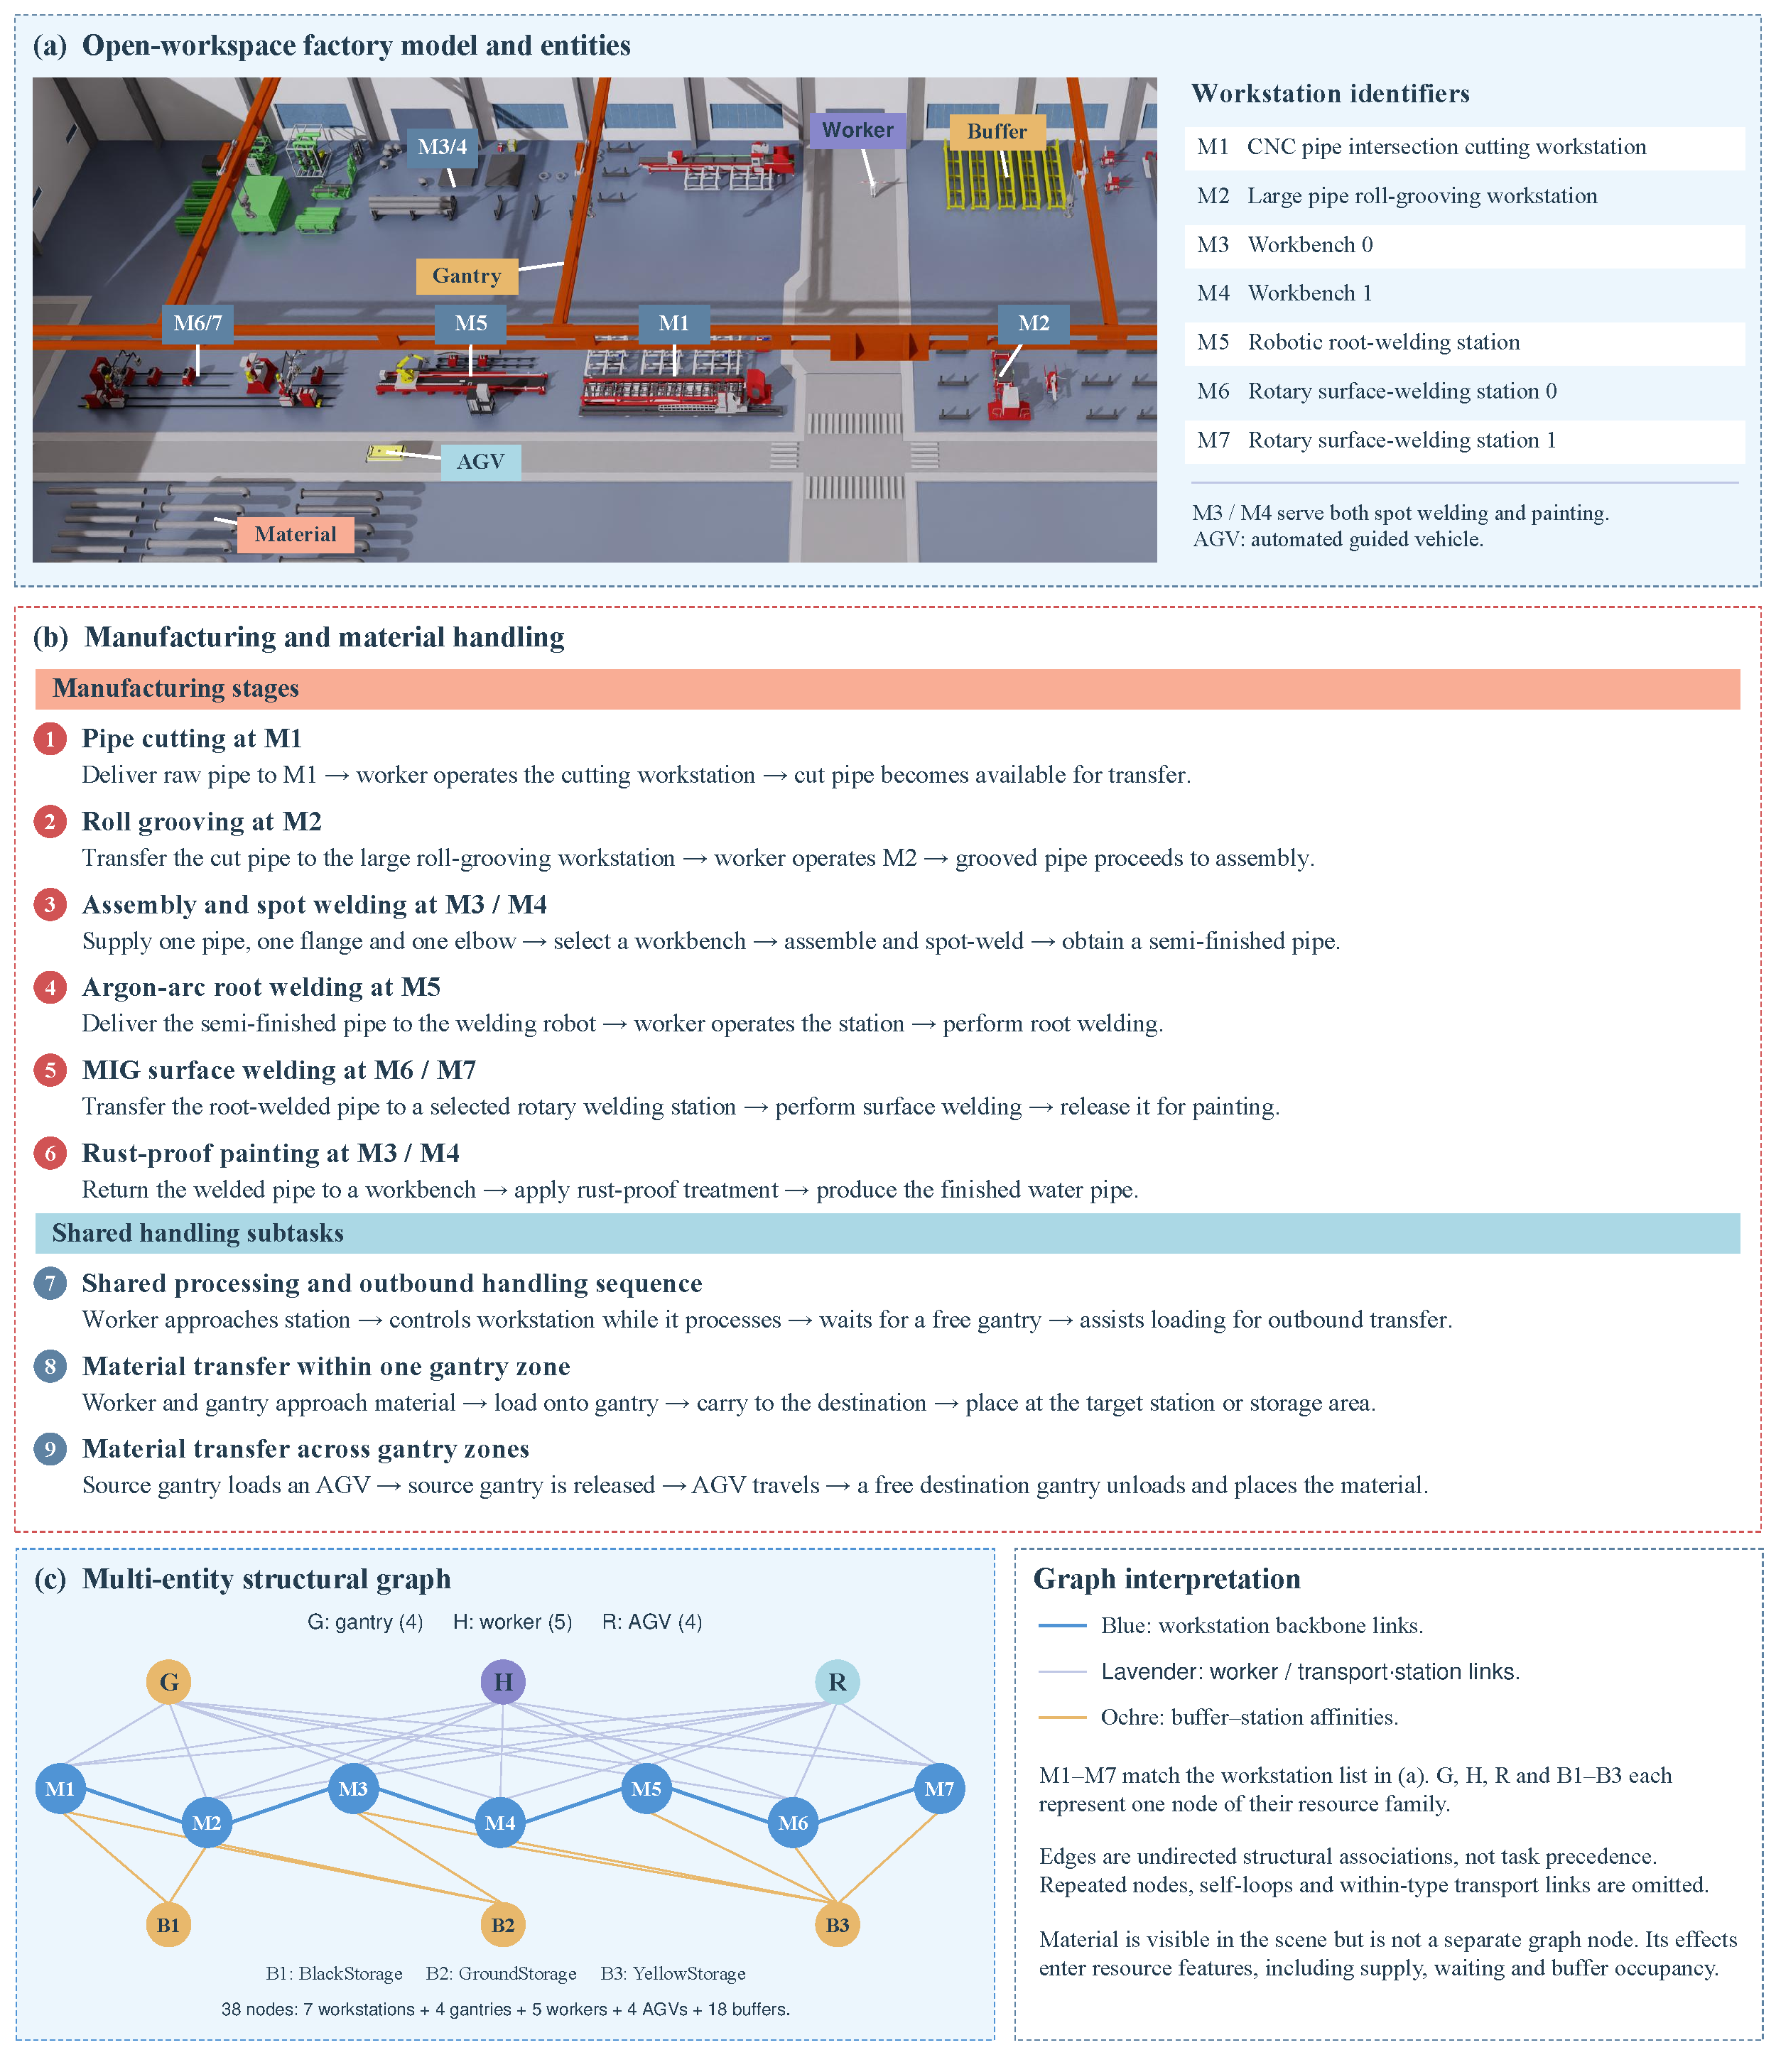
\includegraphics[width=\linewidth]{figures/fig_experiment.pdf}
\caption{Open-workspace factory model developed for NVIDIA Isaac Sim: (a)~resource entities; (b)~manufacturing stages; (c)~structural graph of 38 resources.}
\label{fig:experiment}
\end{figure}

The data-generation environment exposes four operating variation dimensions and applies variations in each dimension at three intervention levels (Table~\ref{tab:disturbance-design}). Level~0 changes episode-wide resource capacity before each model run, Level~1 perturbs sampled processing or service behaviour, and Level~2 injects temporary events during production. The platform supports intensity $I\in\{1,2,3\}$; slash-separated values in the table follow this order. The main \texttt{dense\_i1} collection activates one dimension at a time at $I=1$, while nominal runs keep all dimensions inactive. The injected dimension controls data generation but is not used as the bottleneck or process-cause label.

\begin{table}[!htbp]
\centering
\caption{Four operating variation dimensions and their three intervention levels. Values separated by slashes correspond to $I=1/2/3$. One model step equals one logical second.}
\label{tab:disturbance-design}
\footnotesize
\setlength{\tabcolsep}{3.2pt}
\renewcommand{\arraystretch}{1.12}
\begin{tabularx}{\linewidth}{@{}p{0.13\linewidth}YYY@{}}
\toprule
Dimension & L0: episode configuration & L1: sampled process variation & L2: temporary runtime events \\
\midrule
Workstation & Disable workbench ws1 and rotary-welding ws1 & Processing-time noise $5/10/15$ steps; success rate $0.88/0.76/0.64$; tool wear $15/30/45$ steps per 1,000 steps & $2/(2$--$3)/(3$--$4)$ idle-station failures; additional $1$--$2/2$--$3/3$--$4$ weld or kitting quality-hold windows \\
Worker & Reduce the number of workers from 5 to $3/2/1$ & Service-time scale $1.55/2.10/2.65$; worker-specific skill range $0.8$--$1.4/0.7$--$1.6/0.6$--$1.8$; time noise $12/22/32$ steps & $2/(2$--$3)/(3$--$4)$ temporary absences, applied only when the selected worker is idle \\
Logistics & Reduce the number of AGVs from 4 to $2/1/1$; retain all four zone gantries & Gantry-time scale $1.65/2.30/2.95$ with motion noise $10/18/26$ steps; weak background process variation & $2/(2$--$3)/(3$--$4)$ gantry or AGV freezes; at least one pulse targets an AGV while other vehicles remain active \\
Material & Keep the nominal inventory of ten pipes, flanges, and elbows; no permanent deletion & At steps 400--1,000, temporarily hide $6$--$7/7$--$8/7$--$8$ idle flanges or elbows for $1{,}400$--$2{,}200/2{,}000$--$2{,}700/2{,}500$--$3{,}200$ steps & After the opening shortage, inject $1$--$2/2$--$3/3$--$4$ complementary flange/elbow shortage pulses; pipe blanks are never hidden \\
\bottomrule
\end{tabularx}
\end{table}

For workstation, worker, and logistics operating variations, every Level~2 pulse lasts at least 600 steps and the intensity-specific upper bounds are 900/1,300/1,400 steps. Event targets, start times, counts, and durations are resampled for each episode using a deterministic seed. Adjacent pulses are separated by at least 360 steps, and an event is delayed until an eligible target is idle rather than interrupting an active operation. These controls produce sustained operating variations while avoiding a deterministic one-to-one mapping between an injection and a labelled bottleneck.

A run-stratified, episode-level split gives 140/28/36 training/validation/test episodes from 204 valid episodes, yielding 20,826/4,331/5,354 forecast windows (Table~\ref{tab:exp-dataset}). Preprocessing uses synchronized episode logs; normalization and temporal-pattern prototypes are fitted on the training split only. Invalid episodes affected by the known simulator deadlock are excluded. All comparisons use the same test-window identities, history length, future grid, target resources, and label definitions. Table~\ref{tab:dataset-labels} reports test-label composition. All single-device trajectory comparisons and the case study use the same cutting workstation (\texttt{num02}) from the same test episode; the selection procedure is documented in Appendix~\ref{app:case-details}.

Process-informed labels combine resource-specific operational evidence, filter short runs, and fill one-window internal gaps. At inference, the model uses the observed history rather than retrospective future occupancy. The onset limit is the maximum admissible offset of a newly emerging bottleneck; experiments compare limits of 5, 10, and 15~min. Bottleneck events are required to persist for at least 8~min ($m=8$ one-minute windows), with ongoing events evaluated over their remaining duration. The future label grid remains fixed at 30 windows. Strict report matching uses a three-window onset tolerance; timing errors are reported in minutes. In the label summary below, Upcoming denotes a newly emerging event, Ongoing denotes an event already active at the forecast origin, and No-event denotes a pair with no eligible event.

\begin{table}[!htbp]
\centering
\caption{Dataset and label protocol used in the experiments.}
\label{tab:exp-dataset}
\footnotesize
\setlength{\tabcolsep}{4pt}
\renewcommand{\arraystretch}{1.08}
\begin{tabularx}{\linewidth}{@{}>{\raggedright\arraybackslash}p{\dimexpr 0.30\linewidth + 1cm\relax}@{\hspace{0.03\linewidth}}>{\raggedright\arraybackslash}X@{}}
\toprule
Item & Setting \\
\midrule
Dataset & \texttt{dense\_i1}, 204 valid episodes, 38 resources \\
Split & 140/28/36 episodes; 20,826/4,331/5,354 windows \\
Windowing & 60-s windows; 30 historical + 30 future windows \\
Targets & 15 resources: 7 workstations, 4 gantries, 4 robots \\
Onset limit & $5/10/15$~min \\
Report matching & Three-window onset tolerance \\
\bottomrule
\end{tabularx}
\end{table}

\begin{table}[!htbp]
\centering
\caption{Test-set label composition by onset limit. Counts are window--resource pairs over 5,354 windows $\times$ 15 targets; percentages are shares of all pairs.}
\label{tab:dataset-labels}
\footnotesize
\setlength{\tabcolsep}{3.2pt}
\renewcommand{\arraystretch}{1.08}
\begin{tabularx}{\linewidth}{@{}>{\raggedright\arraybackslash}p{0.24\linewidth}>{\raggedleft\arraybackslash}X>{\raggedleft\arraybackslash}X>{\raggedleft\arraybackslash}X@{}}
\toprule
Onset limit & Upcoming & Ongoing & No-event \\
\midrule
$\leq5$ & 336 (0.42\%) & 766 (0.95\%) & 79,208 (98.63\%) \\
$\leq10$ & 604 (0.75\%) & 768 (0.96\%) & 78,938 (98.29\%) \\
$\leq15$ & 708 (0.88\%) & 770 (0.96\%) & 78,832 (98.16\%) \\
\bottomrule
\end{tabularx}
\end{table}

\subsection{Baseline methods}

Four baselines represent recurrent, graph-based, and Transformer forecasting approaches. LSTM models historical sequences; BSTAN combines graph attention with GRU for blockage/starvation-related prediction~\citep{lai2023bstan}; BTGCN combines production-task graphs with GCN and GRU~\citep{yin2025btgcn}; and PDFormer is adapted from its propagation-delay-aware Transformer architecture for bottleneck prediction~\citep{jiang2023pdformer}. All baselines follow the unified experimental protocol, with architecture-specific input representations and learning algorithms. The validation-only fallback rule is documented in Appendix~\ref{app:additional}.

\begin{table}[!htbp]
\centering
\caption{Baseline models and their roles in the comparison.}
\label{tab:exp-baselines}
\footnotesize
\setlength{\tabcolsep}{4pt}
\renewcommand{\arraystretch}{1.10}
\begin{tabularx}{\columnwidth}{@{}lXX@{}}
\toprule
Model & Core framework & Comparison role \\
\midrule
LSTM & Long short-term memory & Recurrent temporal predictor \\
BSTAN & Graph attention + GRU & Graph-attention predictor \\
BTGCN & Graph convolution + GRU & Graph-convolutional predictor \\
PDFormer & Propagation-delay-aware Transformer & Spatiotemporal Transformer predictor \\
\bottomrule
\end{tabularx}
\end{table}

\subsection{Overall experimental settings and metrics}

All experiments use common data splits, forecast windows, targets, initialization controls, training-budget standards, and validation-based selection. Full and ablation models start from the same fixed parameter state; all selected models and report thresholds are frozen before testing.

Shared PHGST-DM settings appear in Table~\ref{tab:shared-training-protocol}. Training uses AdamW with a batch size of 16, a learning rate of $5\times10^{-5}$, a weight decay of $0.05$, cosine learning-rate decay to $10^{-6}$, and fourfold positive-window oversampling. Under the two-stage training procedure, stage~1 starts from the fixed parameter state shared by all ablation arms, unfreezes all five encoder blocks, and runs for at most 50 epochs with an early-stopping patience of 40. Far-onset weighting doubles onset loss beyond 5~min and uses positive weights $9/10/11$ for the three limits; ordinary and hard false-positive weights are $2.5$ and $2.2$. Stage~2 runs for at most 20 epochs, with the checkpoint selected by validation loss. All runs use seed 42 and provide point estimates rather than multi-seed stability estimates. Appendix~\ref{app:additional} provides loss weights, label thresholds, and decoding details.

The model and report threshold are selected on the validation split. Candidate thresholds are listed explicitly in Table~\ref{tab:shared-training-protocol}; selection uses the internal station-identification F1 among candidates satisfying validation report precision $\geq0.80$ and recall $\geq0.70$. This selection score is not reported as a result; the reported event metric is the onset-qualified F1-score defined below. PHGST-DM uses the selected threshold of $0.94$ for testing at all three onset limits.

For resource $n$ at forecast origin $t$, let $\hat s_{t,n}$ and $s_{t,n}$ denote the predicted and reference onset offsets in minutes. A strict report-level hit requires the correct resource and an absolute onset error within tolerance $\epsilon_s$:
\begin{equation}
|\hat{s}_{t,n}-s_{t,n}|\leq\epsilon_s,\qquad
\epsilon_s=3~\mathrm{min}.
\end{equation}
At the one-minute window resolution, this tolerance equals three windows.

Metrics cover bottleneck-event prediction, process-cause classification, and remaining order time. The reported bottleneck-event F1-score requires both correct station identification and an onset error within three windows. Upcoming recall uses future-event window--resource pairs whose final historical window is non-bottleneck; Ongoing recall uses pairs with an active final historical window. Mean absolute error (MAE) for onset and duration is measured on correctly detected events, while union duration MAE and root mean squared error (RMSE) include missed events and false positives. Event F1 is the harmonic mean of precision and recall; macro recall is the unweighted mean of class-specific recalls. Next-window and 30-window State F1 describe the predicted occupancy over time, including recovery. Process-cause evaluation uses accuracy and macro recall over the four supported classes. Order-completion evaluation uses remaining-time MAE at the line level.

\begin{table}[!htbp]
\centering
\caption{Metrics used in the main evaluation and component analyses.}
\label{tab:exp-metrics}
\footnotesize
\setlength{\tabcolsep}{3.5pt}
\renewcommand{\arraystretch}{1.08}
\begin{tabularx}{\linewidth}{@{}p{0.14\linewidth}p{0.27\linewidth}Y@{}}
\toprule
Group & Metric & Interpretation \\
\midrule
Event & F1-score & Correct station and onset within three windows \\
Warning & Upcoming / ongoing recall & Historically cold / already active resource \\
State & F1 (1 step / horizon) & Occupancy at the next window / across 30 windows \\
Temporal & Onset / duration MAE & Error on correctly detected events \\
Temporal & Union duration MAE/RMSE & Includes missed events and false positives \\
Auxiliary & Remaining-time MAE & Global order-progress error \\
Auxiliary & Cause accuracy / macro recall & Four supported process-cause classes \\
\bottomrule
\end{tabularx}
\end{table}

\FloatBarrier
\section{Overall bottleneck prediction performance}\label{sec:comparison-overview}

This section evaluates how well PHGST-DM jointly predicts bottleneck events, process causes, and remaining order time. Its performance is compared with four baselines under the shared experimental protocol (Tables~\ref{tab:comparison-main}--\ref{tab:comparison-remain}).

\subsection{Bottleneck station, onset, and duration}\label{sec:comparison-event}

At the event level, we assess how accurately PHGST-DM identifies bottleneck stations and predicts their onset, duration, and future occupancy (Table~\ref{tab:comparison-main}).

PHGST-DM achieves the highest event F1, upcoming recall, ongoing recall, and state F1 across the onset limits. Relative to the strongest baseline for each metric and limit, event F1 improves by 8.2--22.1 percentage points and upcoming recall by 28.7--39.9 percentage points. These gains show improved detection before bottlenecks become active, alongside continued coverage of persistent constraints (Figure~\ref{fig:baseline-comparison}).

\begin{table}[!htbp]
\centering
\caption{Bottleneck event and temporal prediction. Scores are percentages except timing MAE (min); best and second-best values are bold and underlined, respectively.}
\label{tab:comparison-main}
\footnotesize
\setlength{\tabcolsep}{3.2pt}
\renewcommand{\arraystretch}{1.12}
\begin{fittable}
\begin{tabular*}{\linewidth}{@{\extracolsep{\fill}}lrrrrrrr@{}}
\toprule
Model & \multicolumn{1}{c}{Event F1 $\uparrow$} & \multicolumn{2}{c}{Event recall $\uparrow$} & \multicolumn{2}{c}{Timing MAE $\downarrow$} & \multicolumn{2}{c}{State F1 $\uparrow$} \\
\cmidrule(lr){2-2}\cmidrule(lr){3-4}\cmidrule(lr){5-6}\cmidrule(l){7-8}
 & F1-score & Upcoming & Ongoing & Onset & Duration & 1 step & 30 steps \\
\midrule
\multicolumn{8}{l}{\textit{Onset limit $\leq5$}} \\
PHGST-DM & \textbf{80.4\%} & \textbf{54.2\%} & \textbf{93.7\%} & 0.127 & \textbf{1.863} & \textbf{88.3\%} & \textbf{52.5\%} \\
LSTM & 58.3\% & 9.9\% & 68.7\% & 0.056 & 3.855 & 29.5\% & 29.5\% \\
BSTAN & 68.7\% & 9.5\% & 79.4\% & 0.043 & 3.565 & 71.9\% & \underline{37.9\%} \\
BTGCN & 66.9\% & 4.6\% & 78.6\% & \underline{0.020} & 3.322 & 64.3\% & 37.2\% \\
PDFormer & \underline{72.2\%} & \underline{14.3\%} & \underline{89.2\%} & \textbf{0.008} & \underline{2.725} & \underline{85.4\%} & 34.7\% \\
\midrule
\multicolumn{8}{l}{\textit{Onset limit $\leq10$}} \\
PHGST-DM & \textbf{77.8\%} & \textbf{53.5\%} & \textbf{93.9\%} & 0.227 & \textbf{1.788} & \textbf{89.2\%} & \textbf{58.9\%} \\
LSTM & 47.7\% & 11.2\% & 69.3\% & 0.388 & 3.768 & 27.5\% & 26.2\% \\
BSTAN & \underline{60.9\%} & 5.7\% & 79.6\% & \underline{0.153} & 3.533 & 63.2\% & \underline{36.5\%} \\
BTGCN & 57.9\% & 4.5\% & 72.2\% & \textbf{0.117} & 3.238 & 56.6\% & 35.9\% \\
PDFormer & 59.8\% & \underline{22.2\%} & \underline{90.2\%} & 0.203 & \underline{2.798} & \underline{84.2\%} & 34.7\% \\
\midrule
\multicolumn{8}{l}{\textit{Onset limit $\leq15$}} \\
PHGST-DM & \textbf{76.8\%} & \textbf{53.7\%} & \textbf{93.0\%} & \underline{0.227} & \textbf{1.716} & \textbf{90.0\%} & \textbf{61.0\%} \\
LSTM & 46.1\% & 10.2\% & 64.3\% & 0.453 & 3.615 & 26.8\% & 26.0\% \\
BSTAN & 53.4\% & 4.4\% & 70.0\% & \textbf{0.222} & 3.422 & 59.3\% & 33.5\% \\
BTGCN & 51.8\% & 5.4\% & 69.9\% & 0.302 & 3.121 & 46.1\% & 32.3\% \\
PDFormer & \underline{54.7\%} & \underline{25.0\%} & \underline{89.5\%} & 0.499 & \underline{2.744} & \underline{82.2\%} & \underline{36.0\%} \\
\bottomrule
\end{tabular*}
\end{fittable}
\end{table}

Detected-event duration MAE is 0.86--1.03~min lower than that of the best baseline at each onset limit, a relative reduction of 31.6--37.5\%. This extends the benefit from identifying an affected station to estimating how long its constraint persists. Timing MAE is conditional on correct detection, and onset MAE alone does not show a uniform advantage over the baselines. Further onset-distance and resource-type results appear in Appendix~\ref{app:supplementary-results}.

\begin{figure}[!htbp]
\centering
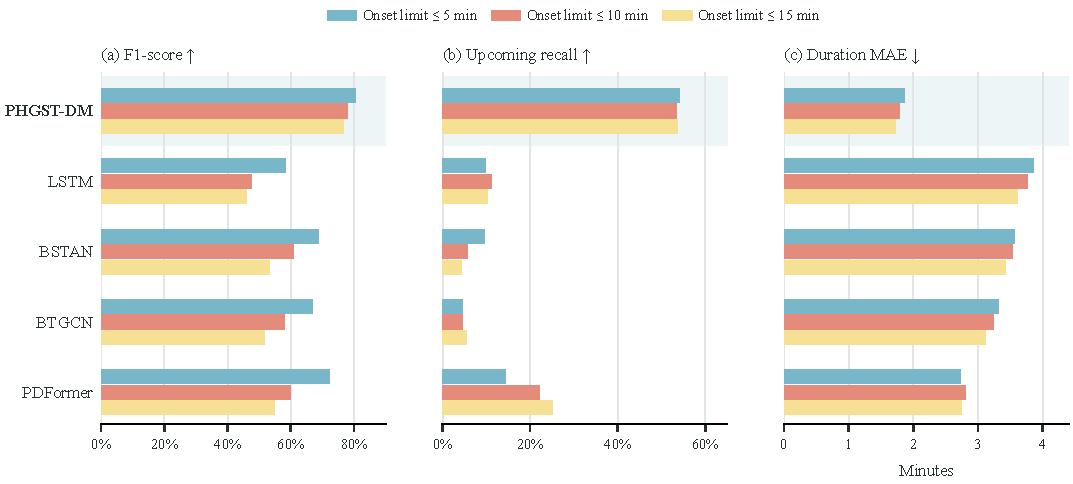
\includegraphics[width=0.96\textwidth,height=0.66\textheight,keepaspectratio]{figures/fig_range_response.pdf}
\caption{Grouped comparison of (a)~F1-score, (b)~Upcoming recall, and (c)~detected-event duration MAE across onset limits.}
\label{fig:baseline-comparison}
\end{figure}

\begin{figure}[!htbp]
\centering
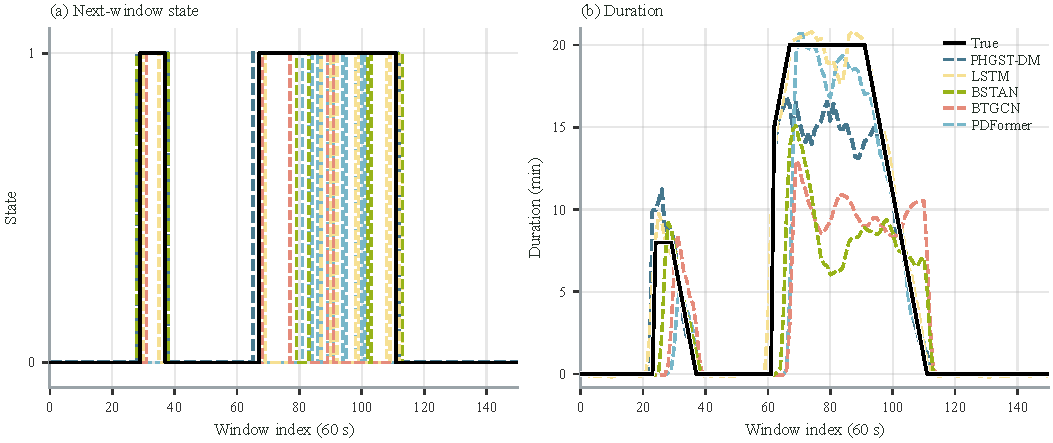
\includegraphics[width=0.90\textwidth,height=0.66\textheight,keepaspectratio]{figures/key_device_models_aligned.pdf}
\caption{Comparison of PHGST-DM and baselines at Onset limit~$\leq5$: (a)~next-window state; (b)~duration with the true reference truncated at 20~min for visualization (black: ground truth; dashed: predictions).}
\label{fig:key-device-baselines}
\end{figure}

Figure~\ref{fig:key-device-baselines} shows the corresponding trajectories. PHGST-DM tracks both bottleneck intervals and the subsequent recovery, connecting event coverage to successive duration forecasts. The displayed true-duration reference is truncated at 20~min, while every model retains the 30-min prediction horizon.

\subsection{Bottleneck process-cause prediction}\label{sec:comparison-cause}

The process-cause comparison covers four operational conditions: material shortage, transport delay, queue buildup, and downstream blockage (Table~\ref{tab:comparison-state}).

PHGST-DM outperforms the four baselines in both cause accuracy and macro recall across the onset limits. Compared with the strongest baseline at each limit, macro recall improves by 1.4--4.3 percentage points.

\begin{table}[!htbp]
\centering
\caption{Bottleneck process-cause prediction (\%). Best and second-best values are bold and underlined, respectively.}
\label{tab:comparison-state}
\footnotesize
\setlength{\tabcolsep}{3.2pt}
\renewcommand{\arraystretch}{1.12}
\begin{fittable}
\begin{tabular*}{\linewidth}{@{\extracolsep{\fill}}lrrrrrr@{}}
\toprule
Model & \multicolumn{2}{c}{Onset limit $\leq5$} & \multicolumn{2}{c}{Onset limit $\leq10$} & \multicolumn{2}{c}{Onset limit $\leq15$} \\
\cmidrule(lr){2-3}\cmidrule(lr){4-5}\cmidrule(l){6-7}
 & Accuracy $\uparrow$ & Macro R $\uparrow$ & Accuracy $\uparrow$ & Macro R $\uparrow$ & Accuracy $\uparrow$ & Macro R $\uparrow$ \\
\midrule
PHGST-DM & \textbf{96.5\%} & \textbf{96.7\%} & \textbf{96.2\%} & \textbf{96.5\%} & \textbf{97.4\%} & \textbf{97.8\%} \\
LSTM & 93.8\% & 92.0\% & 93.6\% & 93.0\% & 94.4\% & 92.2\% \\
BSTAN & \underline{95.7\%} & \underline{95.2\%} & \underline{95.9\%} & \underline{95.1\%} & \underline{95.1\%} & \underline{93.5\%} \\
BTGCN & 90.0\% & 88.2\% & 90.7\% & 90.0\% & 90.7\% & 90.0\% \\
PDFormer & 88.8\% & 88.7\% & 76.9\% & 74.7\% & 79.6\% & 77.3\% \\
\bottomrule
\end{tabular*}
\end{fittable}
\end{table}

\subsection{Order-completion remaining-time prediction}\label{sec:comparison-remain}

After joint training, the remaining-time head is fine-tuned while the encoder and all other prediction heads remain fixed. Table~\ref{tab:comparison-remain} compares the first- and second-stage PHGST-DM predictions with the baselines on the same test windows.

\begin{table}[!htbp]
\centering
\caption{Global order remaining-time MAE (min; lower is better). Best and second-best values are bold and underlined, respectively.}
\label{tab:comparison-remain}
\footnotesize
\setlength{\tabcolsep}{3pt}
\renewcommand{\arraystretch}{1.10}
\begin{fittable}
\begin{tabular*}{\linewidth}{@{\extracolsep{\fill}}lrrr@{}}
\toprule
Model & Onset limit $\leq5$ & Onset limit $\leq10$ & Onset limit $\leq15$ \\
\midrule
PHGST-DM (stage 1) & 10.93 & 11.21 & 9.72 \\
PHGST-DM (stage 2) & \textbf{9.60} & \textbf{9.27} & \textbf{8.91} \\
\midrule
LSTM & 10.59 & \underline{10.61} & \underline{9.01} \\
BSTAN & 14.77 & 13.855 & 13.56 \\
BTGCN & 19.34 & 18.10 & 12.83 \\
PDFormer & \underline{10.437} & 11.254 & 10.422 \\
\bottomrule
\end{tabular*}
\end{fittable}
\end{table}

Second-stage fine-tuning reduces remaining-time MAE by 0.81--1.94~min across the onset limits, equivalent to an 8.3--17.3\% reduction relative to stage~1, while retaining the event and cause outputs.

Figure~\ref{fig:remain-finetune} shows that most of the improvement occurs in the early and middle production phases.

After fine-tuning, PHGST-DM achieves the lowest remaining-time MAE at every onset limit, reducing error by 0.10--1.34~min relative to the strongest baseline at each limit. This combines competitive order-progress estimation with the resource-level event and process-cause forecasts.

\begin{figure}[!htbp]
\centering
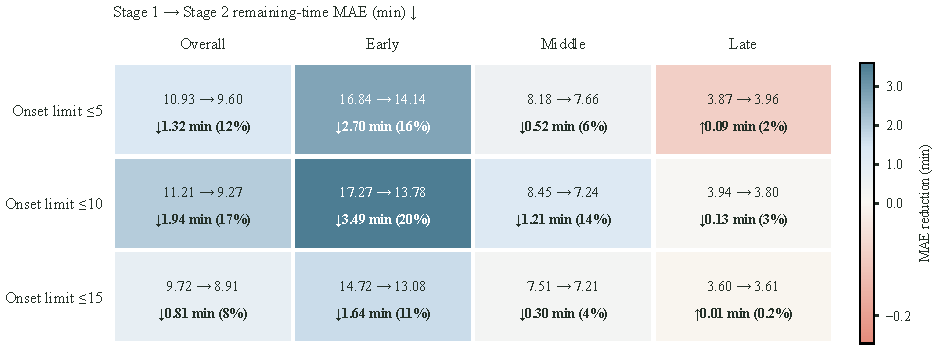
\includegraphics[width=0.90\textwidth,height=0.66\textheight,keepaspectratio]{figures/fig_remain_dumbbell.pdf}
\caption{Effect of remaining-time fine-tuning across early, middle, and late production phases (blue: MAE decrease; coral: increase).}
\label{fig:remain-finetune}
\end{figure}

\FloatBarrier
\section{Evaluation of the proposed components}

The component studies isolate heterogeneous multi-entity representation, process-informed supervision and temporal pattern clustering, and recurrent-pattern-guided delay-aware modelling (Table~\ref{tab:ablation-arms}). Full and all ablation arms share initialization, training budget, curriculum, and validation selection. Remaining-time ablations compare models before head-specific fine-tuning to keep the optimization conditions matched; the fine-tuned full-model results are evaluated in Section~\ref{sec:comparison-remain}. Section~\ref{sec:decoder-training} examines the supporting decoder and training components.

\begin{table}[!htbp]
\centering
\caption{Ablation arms. Every comparison, including the Full reference, begins from identical parameter values and uses the same 50-epoch budget, Onset limit~$\leq5\rightarrow$Onset limit~$\leq10\rightarrow$Onset limit~$\leq15$ curriculum, and validation-controlled model-selection rule.}
\label{tab:ablation-arms}
\footnotesize
\setlength{\tabcolsep}{3.5pt}
\renewcommand{\arraystretch}{1.08}
\begin{tabularx}{\linewidth}{@{}p{0.20\linewidth}p{0.23\linewidth}Y@{}}
\toprule
Arm & Component & Change relative to Full \\
\midrule
NoGraph & Heterogeneous graph & Self-loop adjacency only; no factory edges  \\
NoGroup & Heterogeneous graph & One linear projection of the 27 channels instead of six semantic groups  \\
NoCross & Heterogeneous graph & Within-type edges only; cross-type semantic attention masked  \\
NoInfo & Heterogeneous graph & Only workstations observed; non-workstation features and five coupling channels zeroed  \\
WorkstationOnly & Heterogeneous graph & NoCross and NoInfo combined  \\
NoCluster & Temporal pattern clustering & Temporal pattern clustering removed  \\
NoPattern & \makecell[l]{Delay-aware modelling} & Recent-patch matching to the temporal-pattern prototype bank disabled  \\
NoSplit & Decoder & One shared event-occurrence head for continuing and new events  \\
NoFarBoost & Training & Far-onset weighting and enhanced false-alarm penalty removed  \\
\bottomrule
\end{tabularx}
\end{table}

\subsection{Heterogeneous multi-entity representation}\label{sec:entity-analysis}

Multi-entity ablations assess the contribution of non-workstation observations and cross-resource relations to advance warning. The ablations restrict non-workstation information, cross-type relations, factory edges, or grouped embedding while retaining the same targets (Tables~\ref{tab:ablation-arms} and~\ref{tab:entity-ablation-new}).

\begin{table}[!htbp]
\centering
\caption{Heterogeneous-graph and multi-entity ablation results. Dur. MAE is union error (min); best and second-best values are bold and underlined.}
\label{tab:entity-ablation-new}
\footnotesize
\setlength{\tabcolsep}{3.5pt}
\renewcommand{\arraystretch}{1.05}
\begin{fittable}
\begin{tabular*}{\linewidth}{@{\extracolsep{\fill}}llrrrrr@{}}
\toprule
Arm & \makecell{Onset\\limit} & F1-score & \makecell{Upcoming\\R} & \makecell{Type\\hmean} & \makecell{State F1\\(1 step)} & Dur.\ MAE \\
\midrule
Full & $\leq5$ & \textbf{80.4\%} & \textbf{54.2\%} & \textbf{50.5\%} & \textbf{88.3\%} & \textbf{4.17} \\
NoGraph &  & 74.6\% & 10.4\% & 38.4\% & \underline{87.3\%} & 5.48 \\
NoGroup &  & \underline{75.3\%} & \underline{33.3\%} & \underline{43.2\%} & 83.5\% & \underline{5.11} \\
NoCross &  & 71.6\% & 22.0\% & 39.6\% & 81.2\% & 5.28 \\
NoInfo &  & 64.4\% & 4.9\% & 0.0\% & 69.9\% & 6.66 \\
WorkstationOnly &  & 65.0\% & 3.3\% & 0.0\% & 70.9\% & 6.51 \\
\midrule
Full & $\leq10$ & \textbf{77.8\%} & \textbf{53.5\%} & \textbf{53.0\%} & \textbf{89.2\%} & \textbf{4.38} \\
NoGraph &  & 64.9\% & 6.5\% & 37.6\% & \underline{84.4\%} & 6.46 \\
NoGroup &  & \underline{65.1\%} & \underline{48.5\%} & \underline{45.2\%} & 82.6\% & \underline{6.05} \\
NoCross &  & 57.1\% & 20.7\% & 37.1\% & 75.9\% & 6.60 \\
NoInfo &  & 54.4\% & 2.1\% & 0.0\% & 68.4\% & 7.57 \\
WorkstationOnly &  & 55.9\% & 1.4\% & 0.0\% & 70.8\% & 7.40 \\
\midrule
Full & $\leq15$ & \textbf{76.8\%} & \textbf{53.7\%} & \textbf{53.6\%} & \textbf{90.0\%} & \textbf{4.43} \\
NoGraph &  & \underline{61.2\%} & 3.7\% & 36.0\% & \underline{86.5\%} & 6.57 \\
NoGroup &  & 60.4\% & \underline{43.2\%} & \underline{46.9\%} & 81.9\% & \underline{6.34} \\
NoCross &  & 51.4\% & 31.1\% & 36.5\% & 76.0\% & 6.77 \\
NoInfo &  & 44.1\% & 21.8\% & 0.0\% & 59.6\% & 7.66 \\
WorkstationOnly &  & 53.4\% & 2.1\% & 0.0\% & 70.6\% & 7.46 \\
\bottomrule
\end{tabular*}
\end{fittable}
\end{table}

At Onset limit~$\leq5$, the full representation improves upcoming recall by 50.9 percentage points over WorkstationOnly and by 49.3 points over NoInfo. Removing cross-resource relations or factory edges also weakens distant-event warning (Figure~\ref{fig:cross-resource-evidence}). These comparisons support both the broader observation scope and its relational organization for recognizing constraints that workstation-centred inputs alone fail to reveal.

\begin{figure}[htbp]
\centering
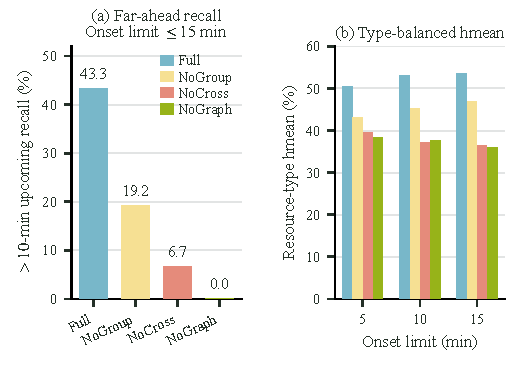
\includegraphics[width=0.82\columnwidth]{figures/fig_cross_resource_evidence.pdf}
\caption{Cross-resource evidence from structural ablations: (a)~far-onset report recall at Onset limit~$\leq15$; (b)~type-hmean F1 across onset limits.}
\label{fig:cross-resource-evidence}
\end{figure}

The complete representation also tracks bottleneck persistence and recovery more closely in Figure~\ref{fig:key-device-entity}. Thus, the heterogeneous graph benefits both advance warning and duration tracking. Resource-level results appear in Appendix~\ref{app:supplementary-results}, with case selection in Appendix~\ref{app:case-details}.

\begin{figure}[!htbp]
\centering
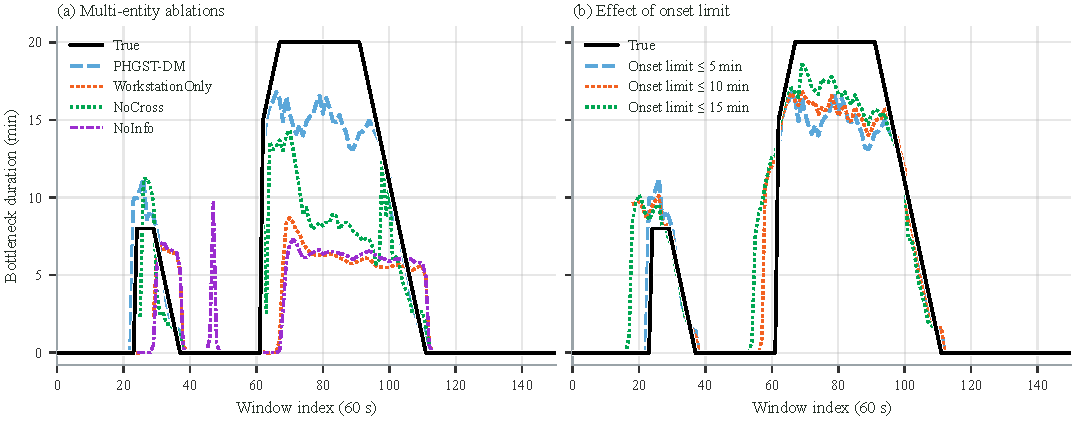
\includegraphics[width=0.96\textwidth,height=0.66\textheight,keepaspectratio]{figures/key_device_entity.pdf}
\caption{Bottleneck-duration traces: panel~(a) compares multi-entity ablations with a 5-min onset limit; panel~(b) compares PHGST-DM with onset limits of 5, 10, and 15~min. The black curve shows the true-duration reference.}
\label{fig:key-device-entity}
\end{figure}

\paragraph*{Cross-resource attention.}\label{sec:attention-protocol}
Figure~\ref{fig:attn-types} examines how the model combines resource information under normal, upcoming, and ongoing bottleneck conditions. Each condition uses 96 episode-stratified test samples, with attention averaged over samples, history steps, heads, and layers. Type-level cells represent mean query-type/attended-type weights. The geographic branch consistently places greater weight on workstations, while the semantic branch exhibits strong workstation--AGV associations and distinct gantry and worker patterns. These associations complement the ablation results by showing how information about production, transport, and workers enters the learned representation. The two branches provide complementary resource views for forecasting constraints whose operational context extends beyond the affected workstation.

\begin{figure}[!htbp]
\centering
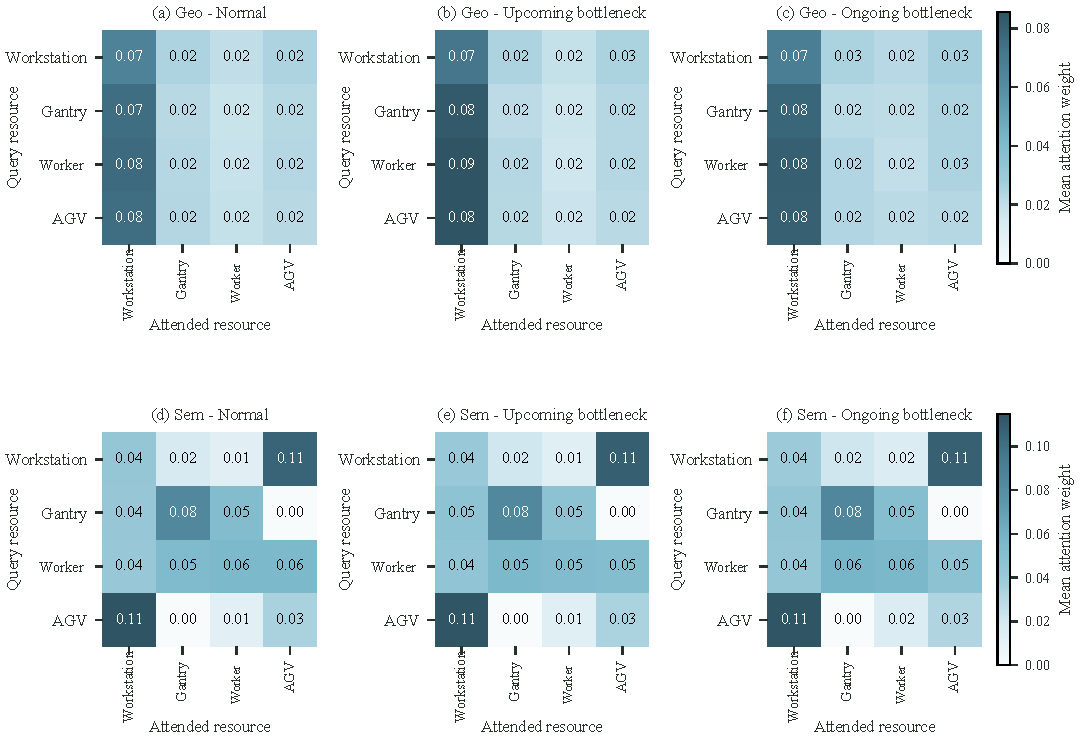
\includegraphics[width=0.92\textwidth,height=0.66\textheight,keepaspectratio]{figures/attention_heatmaps/fig06_entity_type_attention.pdf}
\caption{Type-level attention summary under normal, upcoming, and ongoing conditions (buffers omitted).}
\label{fig:attn-types}
\end{figure}

\subsection{Process-informed supervision and temporal pattern clustering}\label{sec:supervision-analysis}

Three complementary studies address temporal pattern clustering, process-cause supervision, and the production relevance of the constructed event labels.

\paragraph*{(1) Effects of temporal pattern clustering.}
NoCluster tests the predictive value of clustering historical patches into recurrent-pattern prototypes (Table~\ref{tab:group-ablation}); NoPattern separately tests prototype use in Section~\ref{sec:delay-analysis}.

At Onset limit~$\leq15$, temporal pattern clustering improves event F1 by 23.1 percentage points and reduces union duration MAE by 2.22~min relative to NoCluster, a 33.4\% reduction. Gains in upcoming recall and next-window state F1 across the onset limits further show that the pattern bank supports both detection and temporal reconstruction.

\begin{table}[!htbp]
\centering
\caption{Temporal-clustering ablation results. Dur. MAE is union error; Dur. MAE (tp) uses correctly reported events; values are in minutes.}
\label{tab:group-ablation}
\footnotesize
\setlength{\tabcolsep}{3.5pt}
\renewcommand{\arraystretch}{1.08}
\begin{fittable}
\begin{tabular*}{\linewidth}{@{\extracolsep{\fill}}llrrrrr@{}}
\toprule
Arm & \makecell{Onset\\limit} & F1-score & \makecell{Upcoming\\R} & \makecell{State F1\\(1 step)} & Dur.\ MAE & \makecell{Dur. MAE\\(tp)} \\
\midrule
Full & $\leq5$ & \textbf{80.4\%} & \textbf{54.2\%} & \textbf{88.3\%} & \textbf{4.17} & \textbf{1.86} \\
NoCluster & & 73.4\% & 12.5\% & 84.1\% & 5.43 & 2.89 \\
\midrule
Full & $\leq10$ & \textbf{77.8\%} & \textbf{53.5\%} & \textbf{89.2\%} & \textbf{4.38} & \textbf{1.79} \\
NoCluster & & 57.0\% & 34.6\% & 78.9\% & 6.69 & 2.40 \\
\midrule
Full & $\leq15$ & \textbf{76.8\%} & \textbf{53.7\%} & \textbf{90.0\%} & \textbf{4.43} & \textbf{1.72} \\
NoCluster & & 53.7\% & 37.3\% & 81.9\% & 6.65 & 2.30 \\
\bottomrule
\end{tabular*}
\end{fittable}
\end{table}

\paragraph*{(2) Effects of cause supervision.}
The cause-supervision comparison holds labels, data split, onset limit, initialization, seed, and training budget constant (Table~\ref{tab:matched-cause}).

Adding cause supervision improves cause accuracy at the separately selected operating point by 67.0 percentage points and macro recall by 68.2 points, while logged station F1 changes by only 0.2 points.

\begin{table}[!htbp]
\centering
\caption{Matched-budget cause-supervision study at onset limit $\leq5$. Values are percentages.}
\label{tab:matched-cause}
\footnotesize
\setlength{\tabcolsep}{3.5pt}
\renewcommand{\arraystretch}{1.08}
\begin{fittable}
\begin{tabular*}{\linewidth}{@{\extracolsep{\fill}}lrr@{}}
\toprule
Metric & Backbone & +Cause \\
\midrule
Logged station F1 & 73.5\% & 73.3\% \\
Logged cause acc. & 19.5\% & \textbf{89.5\%} \\
Selected cause acc. & 25.2\% & \textbf{92.2\%} \\
Selected cause macro recall & 25.5\% & \textbf{93.7\%} \\
\bottomrule
\end{tabular*}
\end{fittable}
\end{table}

% Evidence: isaac_factory origin/dev_tyx, 8767583f3ed6392cfd8061d4a80de94fcfb9d7a0.
% Source: bottleneck ground-truth validity notes (2026-10-14), checked against label/evaluation code.
% Imported summary values: experiments/data/label_validity_dev_tyx_8767583.json.
\paragraph*{(3) Validation against production sensitivity.}
To assess the production relevance of the event labels, the pilot compares their rankings with order-completion sensitivity under a fixed counterfactual replay protocol. The pilot uses 30 disturbance-free development episodes, separately from predictor training and testing. At a saved factory state, each of seven workstation candidates is accelerated in a separate replay: workstation processing and associated worker-service durations are scaled by $0.8$ (a $1.25\times$ service rate) for 1,200 model steps. Baseline and intervention branches start from the same simulator and random-number states and run to order completion. The reduction in completion time measures production sensitivity. Label methods rank candidates using the preceding three fully observed windows. NDCG@3 measures ranking quality; Positive Recall@$k$ measures top-$k$ coverage; Weighted Recall@3 weights coverage by positive sensitivity; and Coverage@3$_{0.9}$ concerns resources within 90\% of the maximum sensitivity. This fixed acceleration experiment assesses label relevance, not a forecast-guided intervention policy.

\begin{figure}[htbp]
\centering
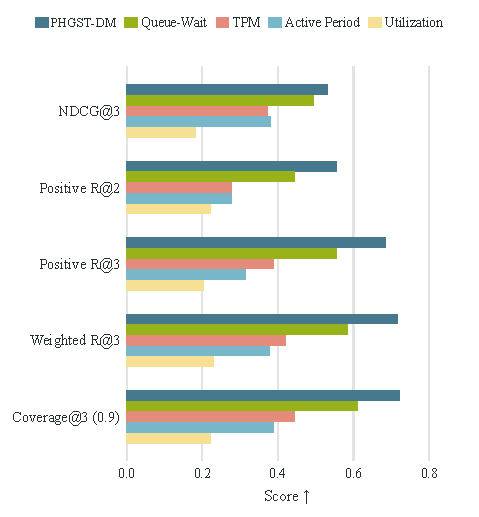
\includegraphics[width=0.76\linewidth,height=0.49\textheight,keepaspectratio]{figures/fig_label_oracle_bars.pdf}
\caption{Counterfactual sensitivity alignment in the exploratory pilot ($\uparrow$: higher is better).}
\label{fig:label-oracle-pilot}
\end{figure}

The process-informed labelling method used by PHGST-DM obtains the highest point estimates on all retained alignment metrics (Figure~\ref{fig:label-oracle-pilot}). Compared with Queue-Wait, NDCG@3 increases by 0.036, Coverage@3$_{0.9}$ improves by 11.1 percentage points, and weighted Recall@3 improves by 13.1 percentage points. Detailed point estimates, reported 95\% confidence intervals for the labelling method, and stage-resolved results are provided in Appendix~\ref{app:supplementary-results}. These exploratory results suggest that combining process evidence helps identify and prioritize resources whose acceleration reduces order-completion time.
\FloatBarrier

\subsection{Delay-aware modelling}\label{sec:delay-analysis}

NoPattern disables recent-patch matching to the fixed prototype bank while retaining the graph and attention branches (Table~\ref{tab:delay-ablation-new}). It isolates historical pattern conditioning from the availability of heterogeneous observations.

At Onset limit~$\leq15$, prototype matching raises strict recall for events more than 10~min ahead by 27.0 percentage points relative to NoPattern, more than doubling distant-event coverage. Improvements in event identification and auxiliary outputs further show that recurrent-pattern conditioning adds forecasting value beyond the heterogeneous graph alone.

This distant-warning benefit supports using earlier resource patterns to anticipate constraints that emerge later, addressing the difficulty of predicting delayed cross-resource effects. Further results appear in Appendix~\ref{app:supplementary-results}.

\begin{table}[!htbp]
\centering
\caption{Temporal-pattern matching ablation in delay-aware modelling. Values compare stage-1 models; onset-distance recall uses strict report matching.}
\label{tab:delay-ablation-new}
\footnotesize
\setlength{\tabcolsep}{2.6pt}
\renewcommand{\arraystretch}{1.08}
\begin{fittable}
\begin{tabular*}{\linewidth}{@{\extracolsep{\fill}}llrrrrrrr@{}}
\toprule
Arm & \makecell{Onset\\limit} & F1-score & \makecell{Upcoming\\R} & $R_{\mathrm{up,rep}}^{6\text{--}10}$ & $R_{\mathrm{up,rep}}^{>10}$ & Queue R & \makecell{Cause\\Macro R} & \makecell{Remain\\MAE} \\
\midrule
Full (stage 1) & $\leq5$ & \textbf{80.4\%} & \textbf{54.2\%} & --- & --- & \textbf{98.4\%} & \textbf{96.7\%} & \textbf{10.93} \\
NoPattern & & 74.5\% & 16.7\% & --- & --- & 14.5\% & 73.4\% & 18.62 \\
\midrule
Full (stage 1) & $\leq10$ & \textbf{77.8\%} & \textbf{53.5\%} & \textbf{46.6\%} & --- & \textbf{98.4\%} & \textbf{96.5\%} & \textbf{11.21} \\
NoPattern & & 58.8\% & 27.8\% & 14.9\% & --- & 47.6\% & 80.5\% & 13.35 \\
\midrule
Full (stage 1) & $\leq15$ & \textbf{76.8\%} & \textbf{53.7\%} & \textbf{52.2\%} & \textbf{43.3\%} & \textbf{98.4\%} & \textbf{97.8\%} & \textbf{9.72} \\
NoPattern & & 60.1\% & 42.7\% & 39.6\% & 16.3\% & 57.3\% & 85.0\% & 11.06 \\
\bottomrule
\end{tabular*}
\end{fittable}
\end{table}

\paragraph*{Historical attention and onset-limit comparisons.}
The descriptive attention maps show that the model draws on multiple historical regions and reweights resource associations across layers and onset limits. The full maps and their interpretation are retained in Appendix~\ref{app:attention-analysis}. These weights describe learned associations and are not evidence of causal effects.

\subsection{Supporting decoder components}\label{sec:decoder-training}

Two decoder-related ablations examine split event heads and far-onset enhancement under the common training and selection protocol (Table~\ref{tab:decoder-ablation}). NoSplit examines the distinction between continuing and newly emerging events; NoFarBoost examines weighting for distant onsets. Each retains its validation-selected operating point.

\begin{table}[!htbp]
\centering
\caption{Split event-head and far-onset ablation results. Thr is the validation-selected threshold; Dur. MAE is union duration error (min).}
\label{tab:decoder-ablation}
\footnotesize
\setlength{\tabcolsep}{3.5pt}
\renewcommand{\arraystretch}{1.08}
\begin{fittable}
\begin{tabular*}{\linewidth}{@{\extracolsep{\fill}}llrrrrrr@{}}
\toprule
Arm & \makecell{Onset\\limit} & Thr & F1-score & \makecell{Upcoming\\R} & $R_{\mathrm{up,rep}}^{>10}$ & \makecell{Ongoing\\R} & Dur.\ MAE \\
\midrule
Full & $\leq5$ & 94.0\% & 80.4\% & 54.2\% & --- & \textbf{93.7\%} & 4.17 \\
NoFarBoost & & 90.0\% & \textbf{81.9\%} & \textbf{54.5\%} & --- & 92.3\% & \textbf{4.03} \\
NoSplit & & 94.0\% & 72.7\% & 19.0\% & --- & 93.5\% & 5.56 \\
\midrule
Full & $\leq10$ & 94.0\% & \textbf{77.8\%} & 53.5\% & --- & 93.9\% & \textbf{4.38} \\
NoFarBoost & & 88.0\% & 75.2\% & \textbf{56.0\%} & --- & 92.3\% & 4.66 \\
NoSplit & & 94.0\% & 58.0\% & 24.7\% & --- & \textbf{94.7\%} & 6.63 \\
\midrule
Full & $\leq15$ & 94.0\% & \textbf{76.8\%} & \textbf{53.7\%} & \textbf{43.3\%} & 93.0\% & \textbf{4.43} \\
NoFarBoost & & 94.0\% & 74.1\% & 48.9\% & 24.0\% & 92.5\% & 4.87 \\
NoSplit & & 94.0\% & 58.6\% & 35.3\% & 12.5\% & \textbf{95.1\%} & 6.36 \\
\bottomrule
\end{tabular*}
\end{fittable}
\end{table}

At Onset limit~$\leq5$, split event heads improve upcoming recall by 35.2 percentage points over NoSplit while retaining high ongoing recall. At Onset limit~$\leq15$, far-onset enhancement raises strict recall beyond 10~min by 19.3 points over NoFarBoost. These gains connect the decoder designs to recognizing newly emerging and more distant events.

Figure~\ref{fig:key-device-struct-graph} shows closer duration tracking by the complete model, with stronger underestimation or post-event spikes in the ablations. Together, the comparisons support decoding that distinguishes current persistence from future onset; weighting benefits remain range-dependent, with NoFarBoost performing better at Onset limit~$\leq5$.

\begin{figure}[!htbp]
\centering
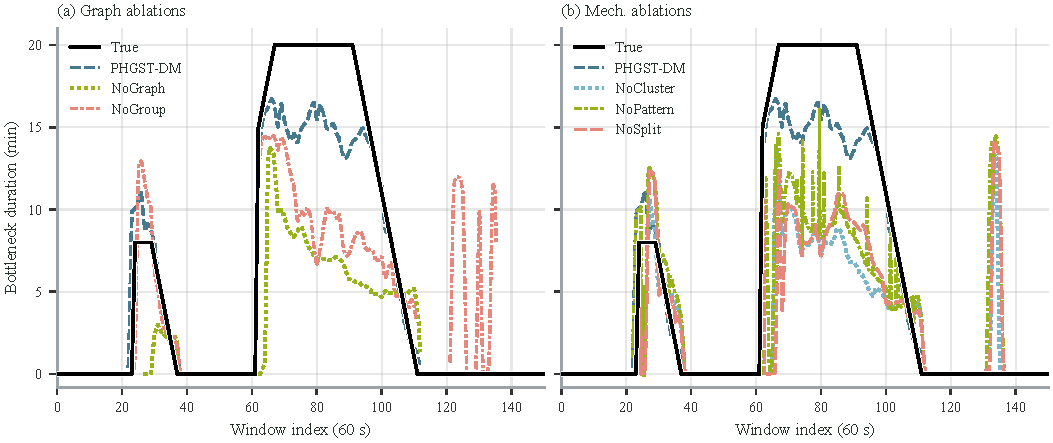
\includegraphics[width=0.96\textwidth,height=0.66\textheight,keepaspectratio]{figures/key_device_struct_pair.pdf}
\caption{Ablation traces (Onset limit~$\leq5$): (a)~graph arms; (b)~process-rule/context, delay-aware modelling, and decoder arms.}
\label{fig:key-device-struct-graph}
\end{figure}

\FloatBarrier
\section{Case study}\label{sec:case-study}

Moving from aggregate results to individual workstation trajectories, the case study assesses predictions of bottleneck onset, duration, and next-window occupancy. The selected episode contains an approximately 8-min bottleneck and a 49-min bottleneck. The prediction horizon is 30~min; the plotted true-duration reference is truncated at 20~min for readability (Figure~\ref{fig:key-device-baselines}). The case is selected by first retaining devices with at least the median event count, then choosing the device with the most events in a single episode, with PHGST-DM one-step F1 breaking ties. Its episode is selected by the number and length of bottleneck segments.

PHGST-DM warns approximately 1~min before the short event, maintains coverage through both intervals, and follows the predicted-duration decline towards recovery. Relative to the baselines, its trajectory contains fewer coverage gaps and follows the sustained constraint more closely (Figure~\ref{fig:key-device-baselines}). Successive forecasts therefore describe bottleneck development through onset, persistence, and recovery.

The workstation state map shows coverage across resources in the same episode (Figure~\ref{fig:all-devices-main}). Full covers the positive cells of both the cutting and second welding workstations, improving episode State F1 by 4.0 percentage points over the strongest ablated configuration, NoGraph. NoInfo and NoCluster miss the welding interval, while NoGraph fragments it. The full model therefore preserves a more complete view of simultaneous workstation constraints within the episode.

% Allow the final experimental figures and Discussion to flow across columns.
\begin{figure}[!htbp]
\centering
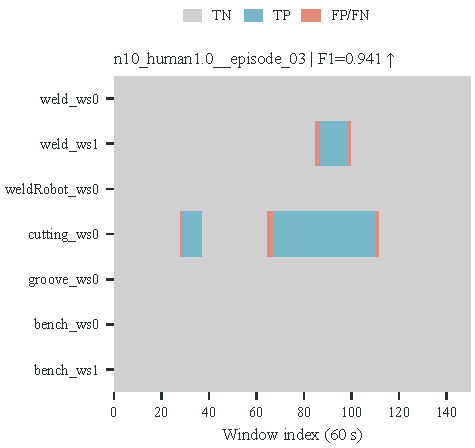
\includegraphics[width=0.82\columnwidth,height=0.66\textheight,keepaspectratio]{figures/all_devices_state_main.pdf}
\caption{Next-window state map for seven workstation targets (grey: TN; light blue: TP; coral: FP/FN). TN, TP, FP, and FN denote true negatives, true positives, false positives, and false negatives, respectively.}
\label{fig:all-devices-main}

\end{figure}



\paragraph*{Resource-level coverage.}
Figure~\ref{fig:per-device} examines whether the joint predictor covers workstations, gantries, and AGVs on the full Onset limit~$\leq5$ test split. Reporting event F1 alongside union duration error separates recognition of an affected resource from reconstruction of its bottleneck interval. The results extend the coverage assessment across resource families and make device-level variation visible instead of hiding it within a single aggregate score.

\begin{center}
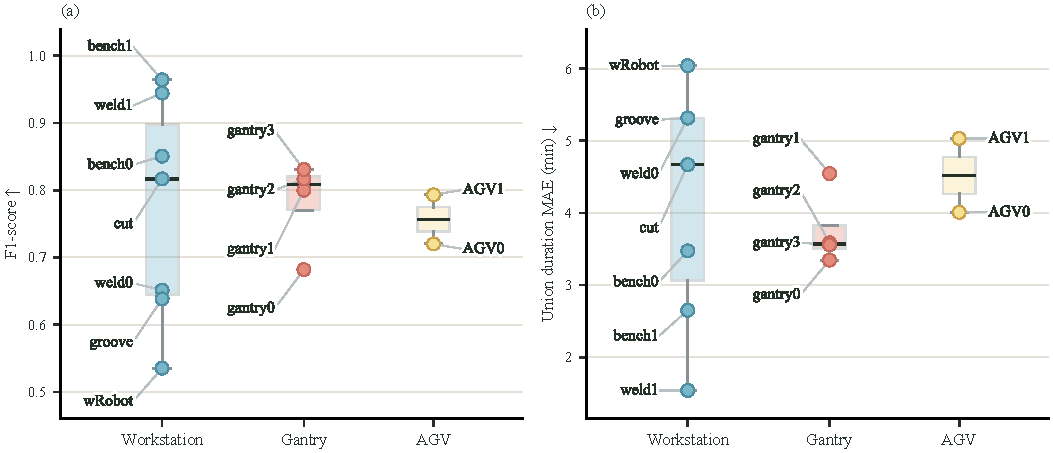
\includegraphics[width=0.95\linewidth,height=0.66\textheight,keepaspectratio]{figures/fig_per_device_box.pdf}
\captionsetup{hypcap=false}
\captionof{figure}{Per-device F1-score and union duration MAE for PHGST-DM at Onset limit~$\leq5$, grouped by resource type: workstation, gantry, and AGV.}
\label{fig:per-device}
\end{center}




% The chapter records implementation challenges and the design responses used in this project.
\chapter{Challenges}
\label{ch:challenges}

Despite the progress, we encountered several challenges during the development and evaluation of the forecasting system. They involved production-system representation, supervision and evaluation, temporal dependencies, and multi-task optimization.

\begin{itemize}[leftmargin=1.7em,itemsep=0.55\baselineskip,topsep=0.35\baselineskip]
\item \textbf{Representing heterogeneous factory resources.} Workstations, workers, buffers, AGVs, gantries, and material-supply observations do not share the same semantics or operational role. Treating them as interchangeable features made it difficult to distinguish a processing constraint from a transport or supply constraint. We addressed this by building a 38-node heterogeneous process--logistics graph, using resource-type projections and semantic feature groups, and keeping geographic and semantic relations separate. The NoGraph, NoGroup, NoCross, and NoInfo ablations helped check whether the representation preserved useful cross-resource information.

\item \textbf{Constructing process-informed bottleneck labels.} The main difficulty was converting noisy process signals into labels that reflect a sustained bottleneck. Queueing, blockage, starvation, worker availability, material shortage, and transport delay can overlap, and a rule that works for a workstation may be inappropriate for a gantry or transport robot. We therefore used resource-specific rules, required at least eight minutes of persistence, filled internal gaps of at most one window, and separated Upcoming from Ongoing events. These choices made the labels more consistent with sustained constraints while keeping them computable from history only.

\item \textbf{Learning from rare events under severe class imbalance.} Roughly 98\% of the test pairs are No-event, so a model can appear accurate by favouring the majority class. At the same time, aggressively recovering the few positive windows can produce unstable false alarms. We mitigated this tension with positive-window oversampling, weighted objectives, far-onset weighting, and a hard-false-positive penalty. Event F1, Upcoming/Ongoing recall, and strict onset matching complemented accuracy.

\item \textbf{Capturing delayed cross-resource effects.} Bottleneck evidence does not always appear first at the resource that will later be affected; changes in an upstream station, transport route, or buffer may become visible elsewhere only after several minutes. This made it difficult to distinguish a meaningful delayed dependency from a short-lived local fluctuation. We addressed the problem with temporal-pattern prototypes and delay-aware cross-resource attention, allowing earlier resource trajectories to condition later predictions. Corresponding ablation experiments were used to assess the effectiveness of these design choices.

\item \textbf{Balancing prediction targets with different scales.} The system had to predict station, onset, duration, cause, and remaining order time at the same time, although these targets have different types, scales, and error costs. A single training schedule could allow one objective to dominate the others or could disturb already useful event outputs when the remaining-time objective was refined. We used two-stage training: Stage~1 jointly learns the shared representation and event-related outputs, while Stage~2 freezes the encoder, event heads, and cause head and fine-tunes only the remaining-time head. This separated the optimization pressures while preserving the event and cause predictions.
\end{itemize}

% Adapted from the manuscript's Discussion and Conclusion; no new empirical claims.
\chapter{Conclusion}
\label{ch:conclusion}

This project presents PHGST-DM for joint bottleneck forecasting in multi-entity production systems. It combines a heterogeneous process--logistics graph, process-informed supervision, and recurrent-pattern-guided delay-aware modelling. The predictor reports the bottleneck station, onset, duration, observable process cause, and remaining order time, connecting resource-level constraints with order-level production progress.

In the evaluated simulation, the model achieves event F1-scores of 80.4\%, 77.8\%, and 76.8\% at onset limits of 5, 10, and 15~min, respectively. These scores exceed the strongest baseline at each limit by 8.2--22.1 percentage points. Detected-event duration MAE is lower by 0.86--1.03~min, equivalent to a 31.6\%--37.5\% reduction. Process-cause accuracy and macro recall also exceed those of the compared baselines. Fine-tuning only the remaining-time head reduces its MAE to 9.60, 9.27, and 8.91~min while retaining the event and cause outputs.

The component studies support complementary roles for the proposed designs. Broader resource observations improve advance-warning coverage; process-cause supervision improves cause identification with little change in logged station F1; and temporal-pattern clustering and prototype matching strengthen the prediction of more distant events. The sensitivity pilot provides preliminary support for label relevance. These findings remain specific to the evaluated simulation; real-factory transfer and the production benefits of forecast-guided interventions require further validation.

Future work will focus on two connected directions. The first is transfer and validation beyond the simulator. Real-factory observations or synchronized digital-twin streams should be combined with the current Isaac Sim data to test sensor noise, incomplete event logs, maintenance periods, operating-speed changes, and production-policy changes. Independently reviewed labels, sensitivity analysis for persistence and threshold choices, rare-event probability calibration, and uncertainty estimates will be needed to determine whether the resource relations and process-informed bottleneck definitions remain reliable. These comparisons can also prioritize the most informative resource signals.

The second direction is forecast-guided operational support. The current predictor reports bottleneck location, onset, duration, cause, and remaining order time, but its outputs are not yet used to change production schedules, reallocate workers or AGVs, or adjust material-transfer orders. Future evaluation should select feasible interventions under resource-capacity, execution-delay, and safety constraints, then measure their effects on bottleneck duration, order completion, and throughput. This will establish a closed loop from prediction to decision, execution, and production response.


% ==================== 参考文献及附录 ====================
% Retain the final manuscript's complete 38-reference set during collaboration.
% After Chapters 1--3 are merged, remove \nocite{*} if only report-cited works are desired.
\nocite{*}
\begingroup
\setstretch{1.10}
\setlength{\bibsep}{6pt}
\bibliographystyle{plainnat}
\bibliography{references}
\endgroup

% Adapted from the manuscript appendices; detailed attention moved from experiments.
\unnumberedchapter{Appendix}
\suppressfloats[t]
\label{ch:appendix}
\setcounter{section}{0}
\renewcommand{\thesection}{\Alph{section}}
\renewcommand{\thesubsection}{\thesection.\arabic{subsection}}
\counterwithin{figure}{section}
\counterwithin{table}{section}
\counterwithin{equation}{section}
\renewcommand{\theHsection}{appendix.\Alph{section}}
\renewcommand{\theHfigure}{appendix.\thesection.\arabic{figure}}
\renewcommand{\theHtable}{appendix.\thesection.\arabic{table}}
\renewcommand{\theHequation}{appendix.\thesection.\arabic{equation}}
\FloatBarrier
\section{Implementation Details and Additional Results}\label{app:additional}

The appendices provide implementation settings, numerical rules, supplementary prediction and case results, and descriptive attention maps.

Table~\ref{tab:shared-training-protocol} summarizes the settings shared by the Full model and ablation arms; their architectural differences are listed in Table~\ref{tab:ablation-arms}.

The exploratory station/window descriptors use eight clusters ($K=8$) and neither define event labels nor contribute a cluster-prediction loss.

\begin{table}[htbp]
\centering
\caption{Shared training, model, and task settings for the Full model and ablation arms.}
\label{tab:shared-training-protocol}
\footnotesize
\setlength{\tabcolsep}{6pt}
\renewcommand{\arraystretch}{1.05}
\begin{tabularx}{\linewidth}{@{}p{0.30\linewidth}Y@{}}
\toprule
Item & Setting \\
\midrule
Initialization and seed & Identical initial parameter values across arms; seed 42 \\
Optimizer and batch size & AdamW; batch size 16; weight decay 0.05 \\
Learning rate & $5\times10^{-5}$ initially; cosine decay to $10^{-6}$ \\
Sampling and training budget & Fourfold positive-window oversampling; at most 50 epochs per onset-limit run; early-stopping patience 40 \\
Curriculum & Onset limit~$\leq5\rightarrow$Onset limit~$\leq10\rightarrow$Onset limit~$\leq15$ \\
Checkpoint criterion & Validation station-identification F1 among candidates with report precision $\geq0.80$ and recall $\geq0.70$ \\
Threshold candidates & $\{0.45,0.50,0.55,0.60,0.65,0.70,0.75,0.80,0.85,0.88,0.90,0.94\}$ \\
Held-out evaluation & Freeze the selected checkpoint and threshold before evaluating the shared test episodes \\
Windowing and targets & 60-s windows; 30 historical and 30 future windows; seven workstation, four gantry, and four transport-robot targets \\
Event and matching rules & One-window internal gap filling; Onset limit~$\leq5/10/15$; three-window onset tolerance \\
Encoder and attention & Five blocks; hidden dimension 80; temporal/geographic/semantic heads $4/2/2$ \\
Graph and positional context & Geographic hop cutoff 4; five semantic neighbours; eight-dimensional Laplacian encoding \\
Pattern bank & 16 prototypes from length-three temporal patches \\
Far-onset enhancement & Onset-loss multiplier 2; positive weights $9/10/11$ for Onset limit~$\leq5/10/15$ \\
False-alarm weighting & Ordinary false-positive weight 2.5; additional hard-false-positive multiplier 2.2 \\
\bottomrule
\end{tabularx}
\end{table}

The joint training objective uses the following weights. Event occurrence, start, duration, and prefix losses have weights $2.4$, $2.0$, $2.0$, and $2.5$, respectively. The cold-history onset term has weight $2.2$ within the event-occurrence objective; focal modulation uses exponent $1.5$, and the internal differentiable F1 term has weight $0.8$. Future occupancy uses separate binary-cross-entropy, Dice, and IoU weights of $0.7$, $0.5$, and $0.35$. The reconstruction, supervised contrastive, cause, and turning-point/momentary losses have weights $0.2$, $0.05$, $0.1$, and $0.25$. Remaining-time regression has weight $0.5$ in stage~1 and $4.0$ during head-only stage~2.

The offline event CSV can retain a one-window event through score-event merging. PHGST-DM training instead constructs targets from the operational occupancy grid.

All state rules act on the original physical feature scale before input standardization. Let $q$, $B$, $S$, $U$, $I$, $R$, and $Z$ denote queue length, blocked seconds, starved seconds, unavailable fraction, inbound-wait seconds, route-delay seconds, and shortage propagation, respectively. At the 60-s resolution, a workstation has raw hot evidence if any of the following holds: (i) $q\geq2$ and $B+S>0$; (ii) $B\geq24$ and $q\geq1$; (iii) $B+S\geq24$ together with an upstream/downstream coupling ratio of at least $0.15$, $I\geq20$, $R\geq20$, $Z\geq0.25$, or $q\geq1$; (iv) $S\geq30$ and $Z\geq0.25$; (v) $S\geq18$ and either $I\geq20$ or $R\geq20$; or (vi) $B+S\geq24$ together with worker absence or labour saturation. An active workstation operating-variation flag combined with $U\geq0.5$ also supplies hot evidence. Worker absence uses unavailable fraction $\geq0.5$; labour saturation uses an activity cutoff of $0.8$ among present workers, with a presence tolerance of $0.05$. A gantry requires $B+S\geq18$ and either $I\geq20$ or $R\geq20$, whereas a transport robot requires $B+S\geq18$ and $I\geq20$; either handling type is also hot when $U\geq0.5$. When an operating-variation flag is active, evidence is retained only if $q\geq1$, $B+S\geq24$, or $U\geq0.5$. Raw indicators are filtered to remove runs shorter than eight one-minute windows, after which internal gaps of at most one window are filled. This retrospective occupancy grid supplies supervision; inference uses only the observed prefix.

For correspondence with the code, the disabled auxiliary-loss switches retain the implementation names \texttt{score}, \texttt{will}, \texttt{mark}, \texttt{time-to-start}, \texttt{STGNPP}, and \texttt{offline cluster-head}. These names identify inactive configuration options; the active occurrence loss $\mathcal{L}_{\mathrm{will}}$ remains part of the training objective. The offline cluster-head weight is zero, so the model is not trained to classify the offline clustering assignments.

The prefix-continuation cutoff is $1.5$ windows. Occupancy-run extraction for event union uses probability cutoff $0.45$, with both ongoing and upcoming union enabled; direct occupancy-state evaluation uses cutoff $0.55$. The configured gantry and transport-robot report thresholds are $0.72$ and $0.68$, respectively, alongside the validation-selected global operating point. Threshold selection first prefers candidates satisfying the validation precision requirement and then maximizes the configured station-identification F1; if none satisfies that requirement, it retains the highest-F1 validation candidate. The checkpoint precision/recall gates are applied separately. If no gated checkpoint is obtained throughout training, the retained ungated checkpoint with the best validation selection score is used. Neither fallback uses test predictions or test labels.

Evaluation counts refer to forecast-origin--resource pairs, so a persistent event may contribute at successive origins. Overlapping windows are not treated as independent observations for significance testing.

\FloatBarrier
\section{Supplementary prediction results}\label{app:supplementary-results}

\subsection{Temporal and resource-type results}

For Onset limit~$\leq15$, strict report recall is $0.574/0.522/0.433$ for onset distances within 5, 6--10, and beyond 10~min. Across the three limit-specific tasks, exact-onset accuracy among station-matched true positives is $0.896/0.844/0.831$, and onset-bucket accuracy is $0.921/0.918/0.920$. Workstation/gantry/robot F1 is $0.805/0.811/0.771$ at Onset limit~$\leq5$ and $0.751/0.840/0.639$ at Onset limit~$\leq15$. Aggregate event and timing results are in Table~\ref{tab:comparison-main}.

\subsection{Structural and pattern-modelling comparisons}

Beyond the main structural-ablation results, NoGroup has a strict report recall of $0.192$ for onsets beyond 10~min. Across limits, resource-type hmean is $0.505$--$0.536$ for Full, $0.360$--$0.384$ for NoGraph, and $0.365$--$0.396$ for NoCross. Figure~\ref{fig:key-device-entity} illustrates the corresponding trajectories: Full identifies both intervals about 5~min before NoInfo and WorkstationOnly, whose duration estimates remain at 6--8~min during the plotted 20-min reference plateau. NoCross reaches 14~min before declining to about 8~min.

\subsection{Stage-resolved sensitivity alignment}

Table~\ref{tab:oracle-pilot-ci} supplements Figure~\ref{fig:label-oracle-pilot} with point estimates and reported 95\% confidence intervals for the Ops labelling method. The results describe the 30-episode development pilot and should be interpreted as exploratory evidence.

% Compact mode is enabled only by the English appendix layout.
\begin{table}[!tbp]

\centering
\caption{Production-sensitivity alignment of the Ops labelling method used by PHGST-DM in the development pilot.}
\label{tab:oracle-pilot-ci}
\footnotesize
\setlength{\tabcolsep}{8pt}

\renewcommand{\arraystretch}{1.1}
\begin{tabular*}{\linewidth}{@{\extracolsep{\fill}}lrrr@{}}
\toprule
Metric & Point estimate & 95\% confidence interval & Interval width \\

\midrule
NDCG@3 & 0.531 & [0.492, 0.570] & 0.079 \\
Positive Recall@2 & 55.556\% & [51.141, 59.971]\% & 8.830 pp \\
Positive Recall@3 & 68.519\% & [63.270, 73.768]\% & 10.497 pp \\
Weighted Recall@3 & 71.623\% & [66.052, 77.194]\% & 11.143 pp \\
Coverage@3$_{0.9}$ & 72.222\% & [66.974, 77.470]\% & 10.497 pp \\
\bottomrule
\end{tabular*}
\par\vspace{3pt}
\begin{minipage}{\linewidth}
\footnotesize
The pilot comprises 30 disturbance-free development episodes. Interval width is the upper bound minus the lower bound; pp denotes percentage points. These exploratory intervals do not establish superiority over the comparison methods or generalization to other disturbance conditions.
\end{minipage}
\end{table}



The mean weighted coverage of positive sensitivity by the top three candidates is $71.6\%$ under the pilot protocol. Early-, middle-, and late-stage NDCG@3 values are $0.421/0.339/0.770$, with the strongest alignment near order completion. 

\FloatBarrier
\section{Case selection and additional resource-level results}\label{app:case-details}

\subsection{Case selection and detailed trace observations}

The episode used for the main case study is \texttt{n10\_human1.0\_\_episode\_03}. The cutting workstation contributes 301 event-positive window--resource pairs. Devices with at least the median event count are first retained. Among them, the device with the most events in a single episode is selected, with ties resolved by PHGST-DM one-step F1. Its episode is then chosen based on the number and length of bottleneck segments. Figure~\ref{fig:key-device-baselines} reports the selected case. PHGST-DM estimates the short-event duration as 10--11~min; during the plotted 20-min reference plateau, estimates are 13--17~min, with state errors spanning 1--2 boundary windows. Plot truncation does not alter the 30-min prediction horizon.

\paragraph*{Mixed-condition probability map.}
Figure~\ref{fig:attn-prediction} uses a supplementary mixed-condition checkpoint and episode \texttt{n10\_mix\_all1.0\_\_episode\_03}, selected automatically for high bottleneck activity. It shows relative test windows $0$--$200$ across 20 rows: 15 target resources and five worker context nodes, omitting 18 buffers. The panels compare future labels, probabilities, and absolute errors. Probabilities are not thresholded reports, and this supplementary configuration does not represent the aggregate performance of the main \texttt{dense\_i1} model.

\begin{figure}[!htbp]
\centering
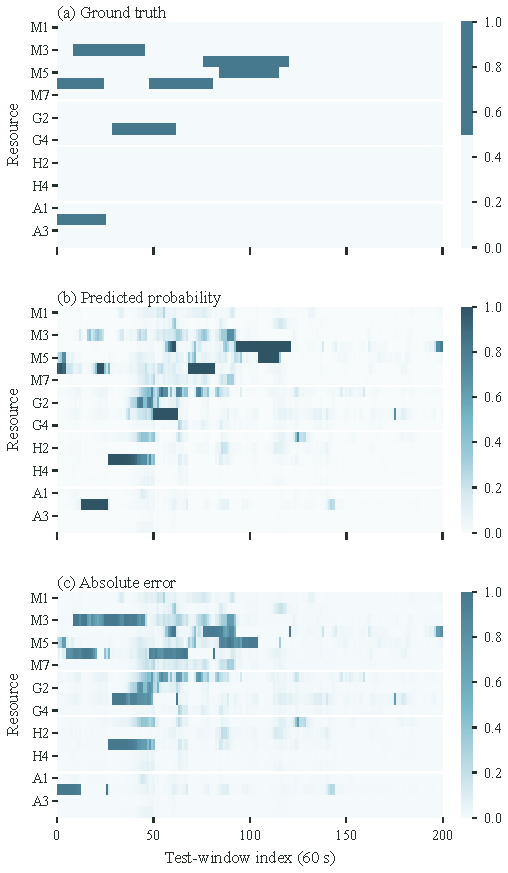
\includegraphics[width=\columnwidth,height=0.55\textheight,keepaspectratio]{figures/attention_heatmaps/fig08_prediction_heatmaps.pdf}
\caption{Future-event labels, predicted probabilities, and absolute errors for a mixed-condition episode (Onset limit~$\leq5$).}
\label{fig:attn-prediction}
\end{figure}

\paragraph*{Resource-level coverage.}

Table~\ref{tab:complete-6-1} provides per-resource counts and errors under the onset-qualified matching rule used in Table~\ref{tab:comparison-main}. Zero-support resources \texttt{robot\_2} and \texttt{robot\_3} are omitted. In this table, $n_{\mathrm{true}}$ and $n_{\mathrm{pred}}$ count reference and predicted event-positive forecast-origin--resource pairs, $P$ and $R$ denote precision and recall, and Dur MAE and Dur RMSE denote union duration errors in minutes. Device identifiers retain the simulator names so individual resources can be traced across data exports.

% Author confirms overall F1 = 80.4 percent and the same matching criterion as the main table.
% Per-device server exports are pending synchronization; do not infer replacement device counts from the aggregate score.
\begin{table}[!tbp]
\centering
\footnotesize
\setlength{\tabcolsep}{3pt}
\renewcommand{\arraystretch}{1.12}
\caption{Per-device event and duration performance at Onset limit~$\leq5$. Durations are in minutes. Zero-support resources (\texttt{robot\_2}, \texttt{robot\_3}) are omitted.}
\label{tab:complete-6-1}
\begin{tabularx}{\textwidth}{@{}lXXXXXXX@{}}
\toprule
Device & $n_{\mathrm{true}}$ & $n_{\mathrm{pred}}$ & $P$ & $R$ & F1-score & Dur MAE & Dur RMSE \\
\midrule
num00\_weld\_ws0 & 115 & 100 & 70.0\% & 60.9\% & 65.1\% & 5.31 & 7.11 \\
num00\_weld\_ws1 & 17 & 19 & 89.5\% & 100.0\% & 94.4\% & 1.54 & 2.76 \\
num01\_robotweld\_ws0 & 46 & 25 & 76.0\% & 41.3\% & 53.5\% & 6.04 & 7.56 \\
num02\_CNC$^\ast$\_ws0 & 301 & 343 & 76.7\% & 87.4\% & 81.7\% & 4.67 & 6.45 \\
num04\_groove\_ws0 & 20 & 27 & 55.6\% & 75.0\% & 63.8\% & 5.32 & 6.87 \\
num08\_bench\_ws0 & 186 & 162 & 91.4\% & 79.6\% & 85.1\% & 3.47 & 5.02 \\
num08\_bench\_ws1 & 94 & 101 & 93.1\% & 100.0\% & 96.4\% & 2.65 & 3.65 \\
gantry\_0 & 18 & 26 & 57.7\% & 83.3\% & 68.2\% & 3.35 & 4.85 \\
gantry\_1 & 31 & 34 & 76.5\% & 83.9\% & 80.0\% & 4.55 & 6.45 \\
gantry\_2 & 108 & 132 & 74.2\% & 90.7\% & 81.7\% & 3.59 & 5.56 \\
gantry\_3 & 121 & 127 & 81.1\% & 85.1\% & 83.1\% & 3.56 & 5.04 \\
robot\_0 & 15 & 10 & 90.0\% & 60.0\% & 72.0\% & 4.01 & 6.14 \\
robot\_1 & 30 & 28 & 82.1\% & 76.7\% & 79.3\% & 5.03 & 6.80 \\
\bottomrule
\end{tabularx}
\end{table}


\FloatBarrier
\section{Supplementary attention analysis}\label{app:attention-analysis}

\subsection{Historical attention and onset-limit comparisons}
Figure~\ref{fig:attn-temporal} compares historical attention under normal and upcoming bottleneck conditions using the protocol in Section~\ref{sec:attention-protocol}. Both maps contain prominent bands around history steps 12--15 and 25--30, indicating that the model draws on multiple historical regions. The upcoming-minus-normal map shows localized increases and decreases around these bands. This pattern is consistent with selective use of historical operating context when forecasting an emerging bottleneck.

\begin{figure}[hbp]
\centering
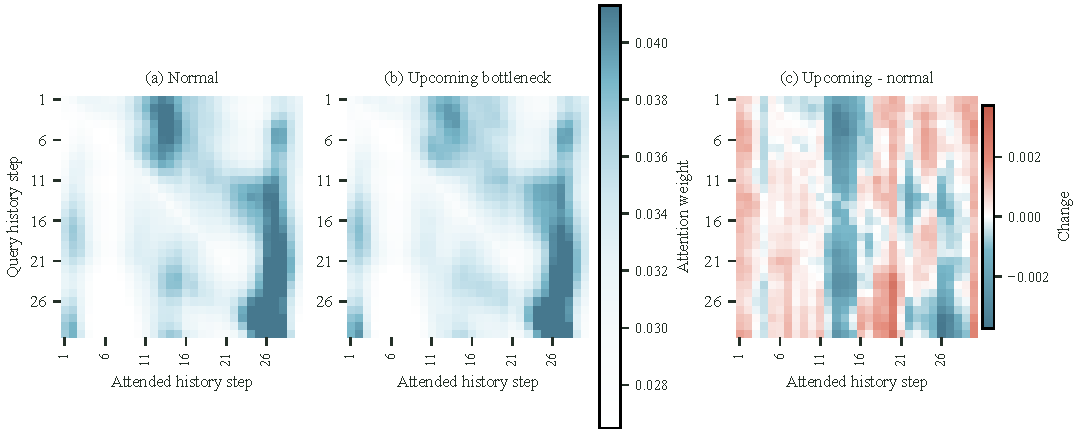
\includegraphics[width=0.98\textwidth,height=0.66\textheight,keepaspectratio]{figures/attention_heatmaps/fig04_temporal_attention_states.pdf}
\caption{Temporal attention over 30 history windows: (a)~normal; (b)~upcoming; (c)~upcoming-minus-normal.}
\label{fig:attn-temporal}
\end{figure}

\begin{figure}[!tbp]
\centering
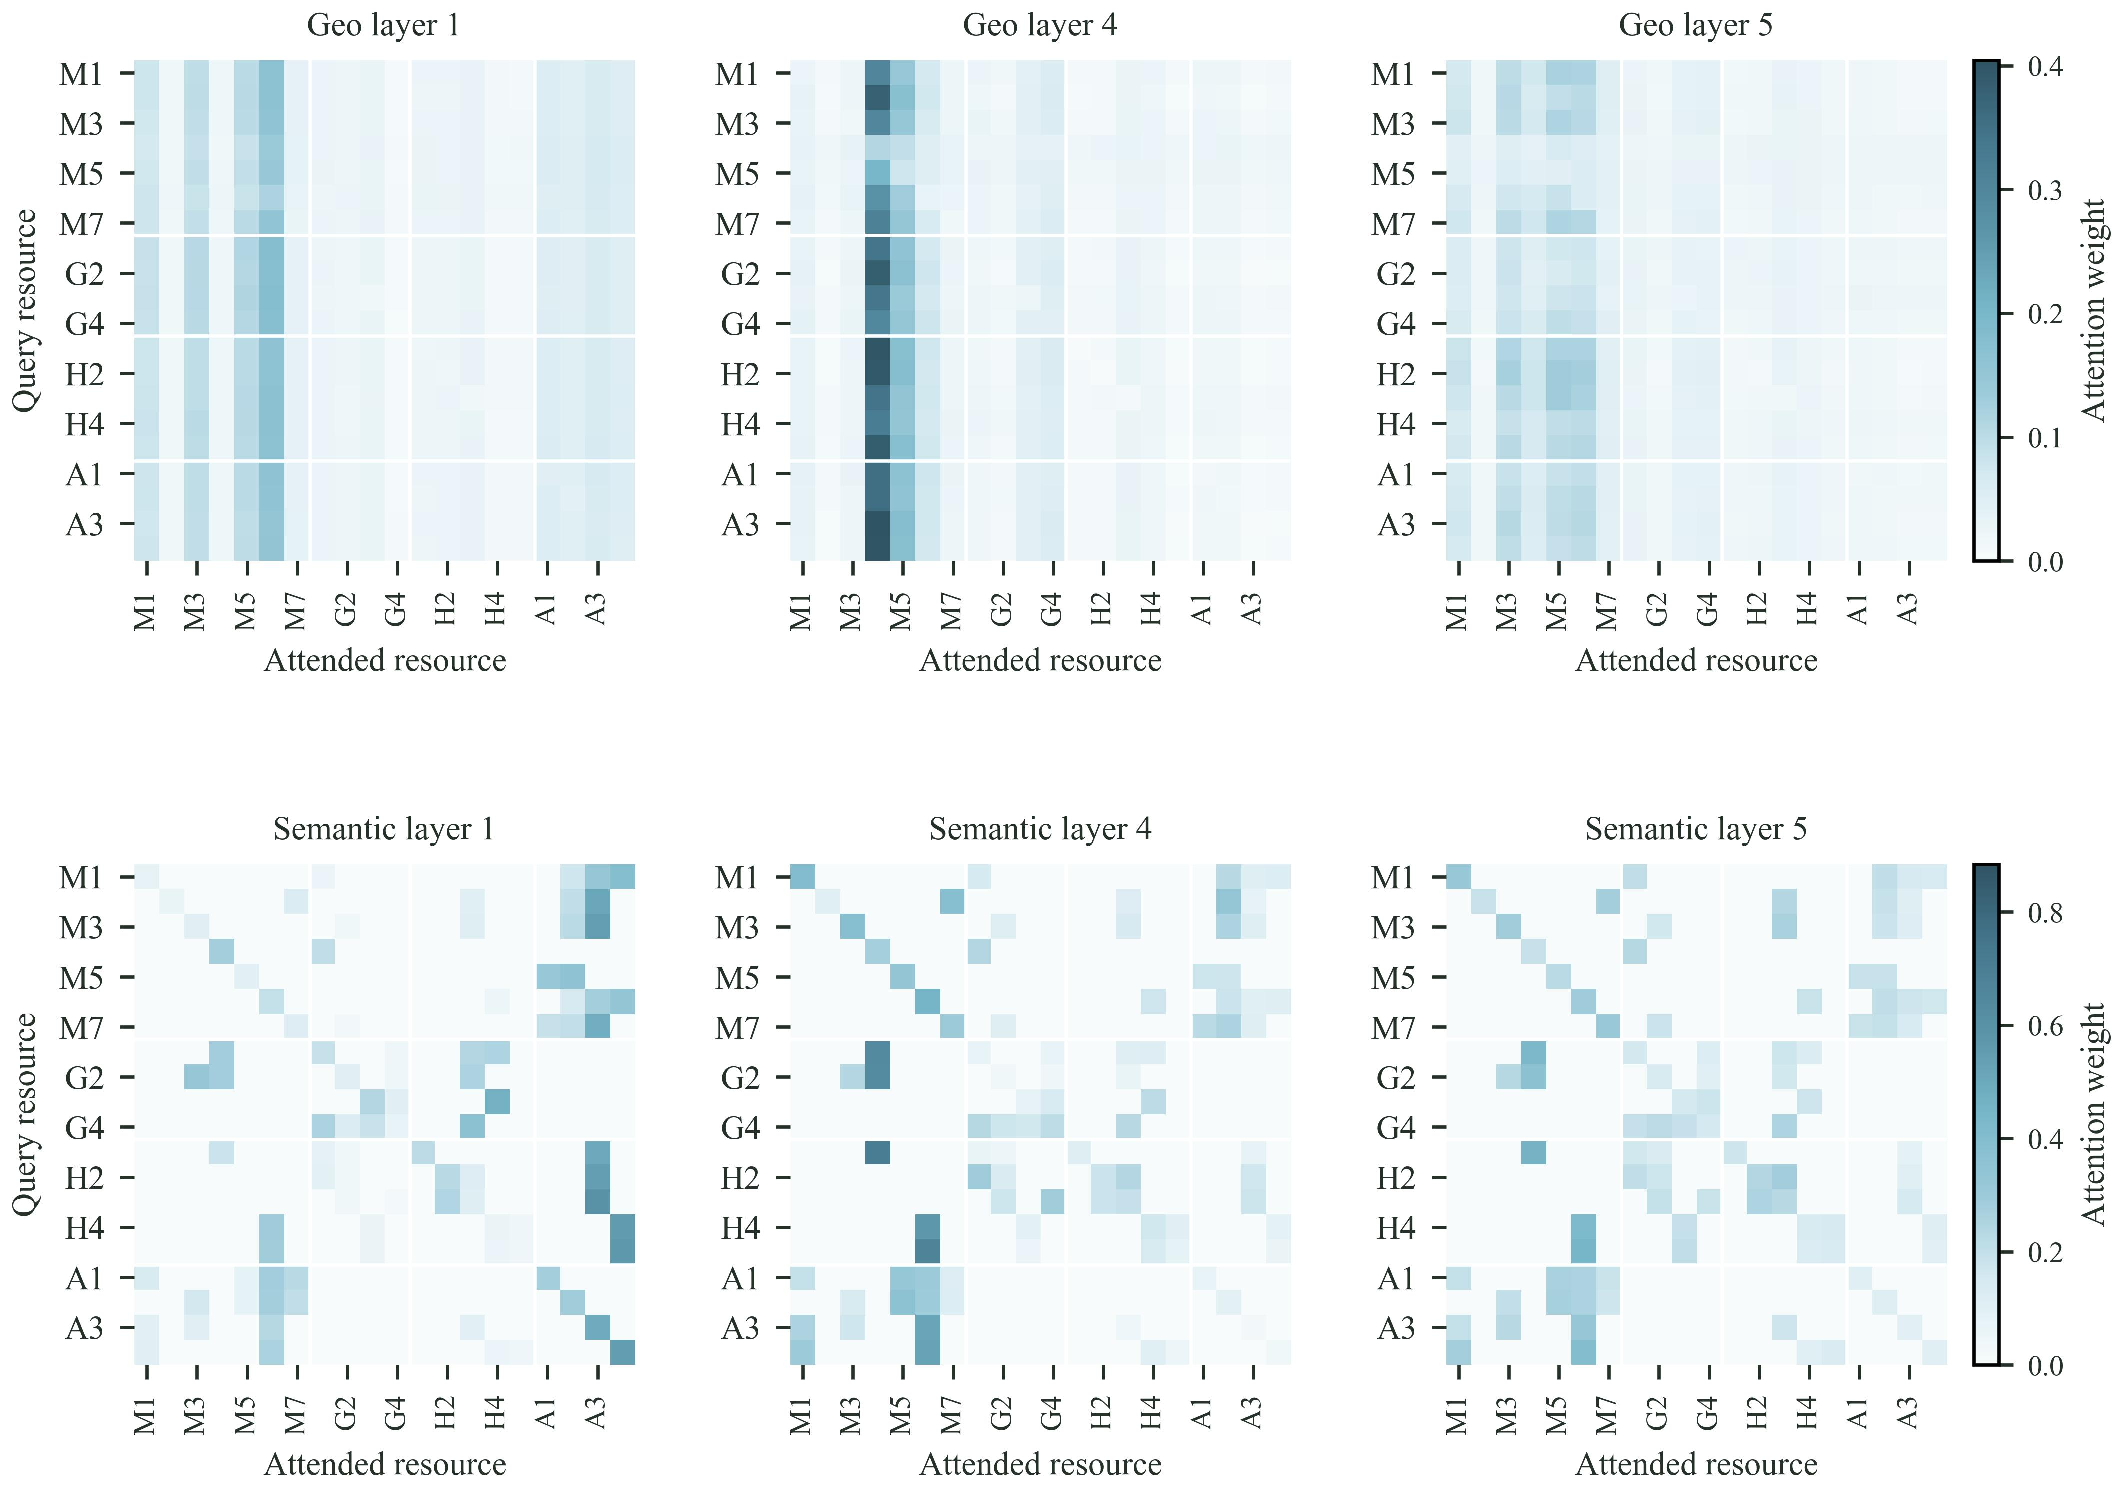
\includegraphics[width=0.92\textwidth,height=0.66\textheight,keepaspectratio]{figures/attention_heatmaps/fig05_layerwise_upcoming_attention_selected.pdf}
\caption{Geographic (upper) and semantic (lower) attention in selected encoder layers 1, 4, and 5.}
\label{fig:attn-layers}
\end{figure}

Figure~\ref{fig:attn-layers} reveals complementary changes across encoder layers. Geographic attention is distributed across several workstation columns in layer~1, becomes concentrated around M3 in layer~4, and is more distributed again in layer~5. Semantic attention remains sparse and resource-specific, with prominent links involving workstations, workers, and AGVs. Together, these views show that resource information is reweighted across layers and combined through distinct geographic and semantic patterns. Appendix~\ref{app:layerwise-attention} presents all five layers.

Figure~\ref{fig:attn-horizons} compares upcoming-minus-normal resource attention under Onset limit~$\leq5/10/15$, using 96 samples per condition. Geographic maps retain a common emphasis on the M3--M5 workstation region, while the magnitudes and extent of the changes vary across onset limits. Semantic maps show localized positive and negative changes, including recurring links to M3--M4 across resource types. Thus, the models share recurring resource associations while adjusting the allocation of attention to the admissible onset range.

\begin{figure}[!tbp]
\centering
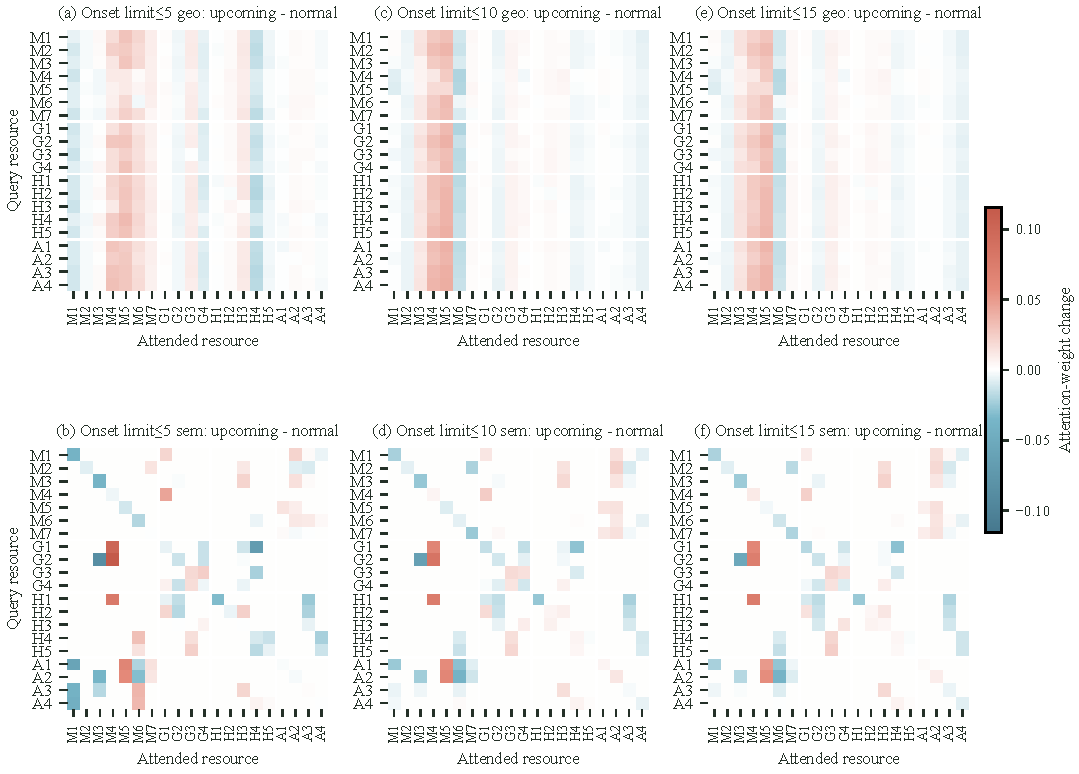
\includegraphics[width=0.98\textwidth,height=0.66\textheight,keepaspectratio]{figures/attention_heatmaps/fig07_horizon_attention_change.pdf}
\caption{Upcoming-minus-normal attention change across onset limits 5/10/15 (upper: geographic; lower: semantic).}
\label{fig:attn-horizons}
\end{figure}

\paragraph*{Learned cross-resource allocation under mixed operating conditions.}
Attention sampling and averaging follow the protocol in Section~\ref{sec:attention-protocol}. Figure~\ref{fig:attn-change} presents the resource-level change maps underlying the type-level summary in the main text.

Average attention under upcoming and ongoing conditions is compared with that under normal conditions. Colour indicates increased or decreased weight; the absolute reference matrices are retained below.

\begin{figure}[!htbp]
\centering
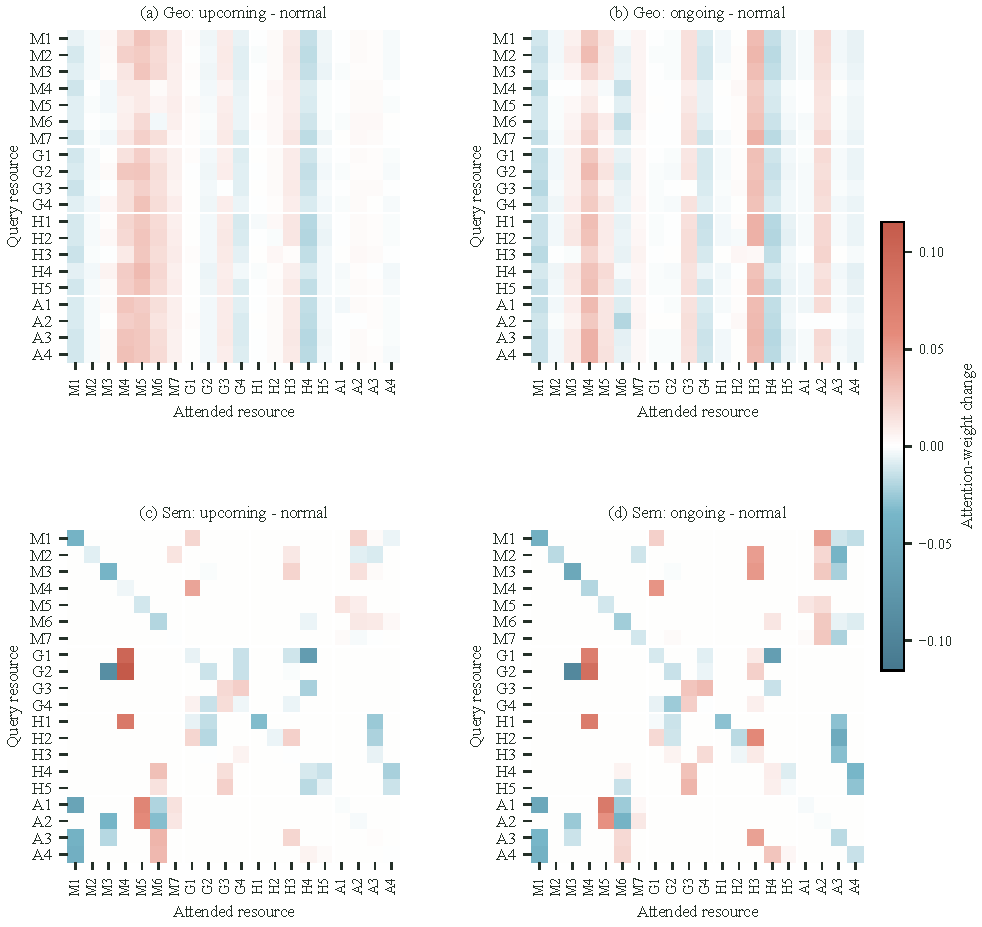
\includegraphics[width=0.92\textwidth,height=0.66\textheight,keepaspectratio]{figures/attention_heatmaps/fig03_resource_attention_change.pdf}
\caption{Redistribution of resource attention under upcoming and ongoing conditions relative to normal conditions (coral: increase; blue: decrease).}
\label{fig:attn-change}
\end{figure}



\subsection{Complete resource and layer matrices}
\label{app:absolute-attention}
\label{app:layerwise-attention}
Figures~\ref{fig:attn-states} and~\ref{fig:attn-layers-all} retain the absolute resource averages and all five layers corresponding to the selected views in this appendix. Layer-wise matrices share the same scale within each branch. Attention weights describe learned associations, not causal effects or layer-wise accuracy contributions.

\begin{figure}[!tbp]
\centering
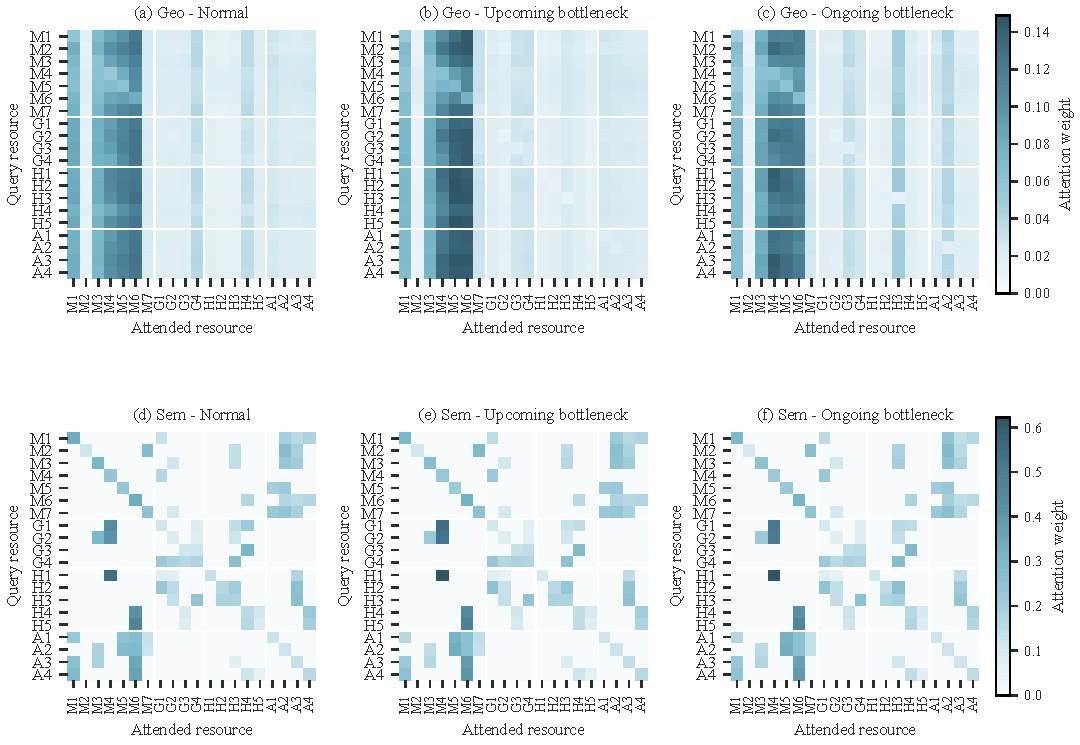
\includegraphics[width=0.92\textwidth,height=0.66\textheight,keepaspectratio]{figures/attention_heatmaps/fig02_resource_attention_states.pdf}
\caption{Absolute geographic (upper) and semantic (lower) resource attention under normal, upcoming, and ongoing conditions.}
\label{fig:attn-states}
\end{figure}

\begin{figure}[!tbp]
\centering
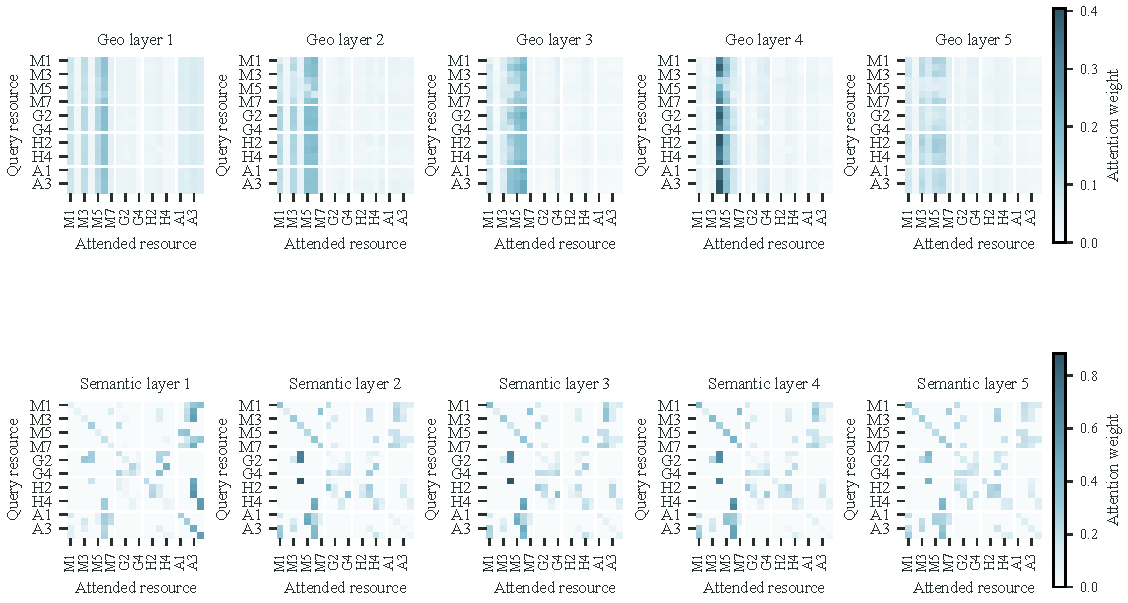
\includegraphics[width=0.94\textwidth,height=0.66\textheight,keepaspectratio]{figures/attention_heatmaps/fig05_layerwise_upcoming_attention.pdf}
\caption{Geographic (upper) and semantic (lower) attention across encoder layers 1--5 for upcoming samples.}
\label{fig:attn-layers-all}
\end{figure}



% ==================== 可选：工作分工表 ====================
% 按参考 PDF 的实际顺序放在最后。以下为可编辑重排版，不是官方原表。
% 参考 PDF 内表格说明提到致谢后放置；最终位置按你的课程要求调整。
% 签名与日期留空，由成员自行填写。
\ifincludeworkdistribution
\clearpage
\thispagestyle{empty}
\phantomsection
\addcontentsline{toc}{chapter}{Work Distribution Form}
\begingroup
\setstretch{1.0}
\begin{center}
  THE UNIVERSITY OF HONG KONG\\[2pt]
  DEPARTMENT OF MATHEMATICS,\\[2pt]
  DEPARTMENT OF STATISTICS AND ACTUARIAL SCIENCE \&\\[2pt]
  DEPARTMENT OF COMPUTER SCIENCE\\[14pt]
  \textbf{\CourseName}\\[4pt]
  \textbf{Work Distribution Form}
\end{center}
\vspace{12pt}
\noindent\textbf{I. WORK DISTRIBUTION}\par
\vspace{8pt}
\noindent Record each member's responsible chapters or project components.
For shared work, specify each member's contribution percentage.\par
\vspace{12pt}
\renewcommand{\arraystretch}{1.2}
\noindent\begin{tabularx}{\linewidth}{|p{0.25\linewidth}|Y|}
  \hline
  \textbf{Name} & \textbf{Responsible Chapters / Parts (\%)} \\
  \hline
  1.\rule{0pt}{25mm} & \\
  \hline
  2.\rule{0pt}{25mm} & \\
  \hline
  3.\rule{0pt}{25mm} & \\
  \hline
  4.\rule{0pt}{25mm} & \\
  \hline
\end{tabularx}
\vspace{22pt}

\noindent\textbf{II. STUDENTS' SIGNATURE}\par
\vspace{18pt}
\noindent\begin{tabularx}{\linewidth}{@{}XX@{}}
  1. \hrulefill & 2. \hrulefill \\[20pt]
  3. \hrulefill & 4. \hrulefill
\end{tabularx}
\vspace{18pt}

\noindent Date: \rule{0.42\linewidth}{0.4pt}
\endgroup
\fi

\end{document}
